\documentclass{article}
\usepackage[english]{babel}
\usepackage{geometry,amsmath,graphicx,xcolor}
\geometry{letterpaper}
%\geometry{b4paper}

%%%%%%%%%% Start TeXmacs macros
\catcode`\>=\active \def>{
\fontencoding{T1}\selectfont\symbol{62}\fontencoding{\encodingdefault}}
\newcommand{\tmaffiliation}[1]{\\ #1}
\newcommand{\tmcolor}[2]{{\color{#1}{#2}}}
\newcommand{\tmop}[1]{\ensuremath{\operatorname{#1}}}
\newcommand{\tmtextit}[1]{{\itshape{#1}}}
%%%%%%%%%% End TeXmacs macros

\begin{document}

\title{Guiding center motion in tokamaks}

\author{
  Youjun Hu
  \tmaffiliation{Institute of plasma physics, Chinese Academy of Sciences\\
  Email: yjhu@ipp.cas.cn}
}

\maketitle

\begin{abstract}
  This note discusses numerical computation of guiding center orbits in
  tokamaks using the cylindrical coordinates and several magnetic coordinates.
  Some subtle things involved in using a particlular kind of magnetic
  coordinates called field-line-following coordinates are discussed (I am
  using this kind of coordinates in developing a new module in GEM code). We
  assume a general tokamak magnetic field speccified numerically (provided by
  the EFIT G-file). This note is evolving, begining with my first try of
  computing guiding-center motion in Solovev analytical equilibrium using
  cylindrical coordinates, and then extending to general numerical magnetic
  field, and later using magnetic coordinates.
\end{abstract}

\

\section{\label{5-15-e1}Equations of guiding-center motion}

The equations of guiding center motion are written{\cite{todo2006}} (refer to
my notes ``collisionless\_drift\_kinetic\_equation.tm'' for the derivation)
\begin{equation}
  \label{5-15-p2} \frac{d\mathbf{X}}{d t} \equiv \mathbf{v}_d =
  \frac{\mathbf{B}^{\star}}{B^{\star}_{\parallel}} v_{\parallel} +
  \frac{\mu}{m \Omega B^{\star}_{\parallel}} \mathbf{B} \times \nabla B +
  \frac{1}{B B^{\star}_{\parallel}} \mathbf{E} \times \mathbf{B}
\end{equation}
\begin{equation}
  \label{16-7-4-7} \frac{d v_{\parallel}}{d t} = - \frac{\mu}{m} 
  \frac{\mathbf{B}^{\star}}{B^{\star}_{\parallel}} \cdot \nabla B + \frac{Z
  e}{m}  \frac{\mathbf{B}^{\star}}{B^{\star}_{\parallel}} \cdot \mathbf{E}
\end{equation}
where $\mathbf{X}$ is the guiding-center position, $v_{\parallel}$ is the
parallel (to the magnetic field) velocity, $m$ and $Z e$ are the mass and
charge of the particle, respectively, $\mu$ is the magentic moment defined by
$\mu = m v_{\perp}^2 / (2 B)$ with $v_{\perp}$ being the pependicular speed;
$\Omega = B Z e / m$ is the cyclotron angular frequency, \
$\mathbf{B}^{\star}$ and $B^{\star}_{\parallel}$ are defined by
\begin{equation}
  \mathbf{B}^{\star} =\mathbf{B}+ B \frac{v_{\parallel}}{\Omega} \nabla \times
  \mathbf{b},
\end{equation}

\begin{equation}
  \label{5-15-p8} B^{\star}_{\parallel} \equiv \mathbf{b} \cdot
  \mathbf{B}^{\star} = B \left( 1 + \frac{v_{\parallel}}{\Omega} \mathbf{b}
  \cdot \nabla \times \mathbf{b} \right),
\end{equation}
respectively, where $\mathbf{b}=\mathbf{B}/ B$. If using approximation
$B_{\parallel}^{\star} \approx B$, then
\begin{equation}
  \frac{d\mathbf{X}}{d t} = v_{\parallel} \mathbf{e}_{\parallel} +\mathbf{V}_D
  = v_{\parallel} \mathbf{b}+ \underbrace{\frac{v_{\parallel}^2}{\Omega}
  \nabla \times \mathbf{b}}_{\tmop{curvature} \tmop{drift}} +
  \underbrace{\frac{\mu}{m \Omega B} \mathbf{B} \times \nabla B_0}_{\nabla B
  \tmop{drift}} + \underbrace{\frac{1}{B^2} \mathbf{E} \times \mathbf{B}}_{E
  \times B \tmop{drift}} .
\end{equation}
[Before getting to know the above form of the equations of the guiding-center
motion, I used the following form of the equations (refer to my notes \
``collisionless\_drift\_kinetic\_equation.tm''):
\begin{equation}
  \frac{d\mathbf{X}}{d t} =\mathbf{b}v_{\parallel} + \frac{1}{\Omega}
  \mathbf{b} \times \left( \frac{\mu}{m} \nabla B + v_{\parallel}^2
  \mathbf{\kappa}- \frac{Z e}{m} \mathbf{E} \right),
\end{equation}
\begin{equation}
  \frac{d v_{\parallel}}{d t} = - \frac{\mu}{m} \mathbf{b} \cdot \nabla B +
  \frac{v_{\parallel} \mu}{m \Omega} \mathbf{\kappa} \cdot \mathbf{b} \times
  \nabla B + \frac{Z e}{m} \mathbf{b} \cdot \mathbf{E},
\end{equation}
which does not converve the toroidal angular momentum $P_{\phi}$ excatly in an
axisymmetrical equilibrium magnetic field (this has been tested numerically)
while the new form given in Eqs. (\ref{5-15-p2})-(\ref{5-15-p8}) can conserve
$P_{\phi}$ excatly. Besides to be more accurate, the new form is compact and
convenient for numerical implementation.] My latest numerical code uses Eqs.
(\ref{5-15-p2})-(\ref{5-15-p8}) as the the equations of guiding center motion.

\subsection{\label{5-17-1}Define new units}

The above formulas are in SI units, which are good since SI units are getting
widely used, and thus these formulas are accessible to most people. However
there is a convention in mathematical physics to define new units for every
particular problem and write formulas in terms of these new units. This
process is often called normalization. This has the advantage of possibly
reducing the numbe of free parameters in a prolem. Another advantage is that,
by chosen proper characteristic quantites as units, the magnitude of quanties
in terms of the new units are easier to be appreciated. A third advantage,
which is usually not important, is that the magnitude of normalized quantities
may be in the vicinity of 1 and thus avoid possible numerical overflow in a
numerical computionation.

The disadvantages of the normalization are the additional work associated with
performing the transformation between the two units systems and possible
confusions associated with the exact units used in a numerical code and the
potential of introducing bugs due to this confusion when writing numerical
codes.

Choose a characteristic magnetic field strength $B_n$ and a characteristic
length $L_n$. Using $B_n$ and $L_n$, we define a characteristic time $t_n
\equiv 2 \pi / \Omega_n$, where $\Omega_n = B_n | Z e | / m$, a characteristic
velocity $v_n = L_n / t_n$, \ and a characteristic magnetic moment $\mu_n = m
v_n^2 / B_n$. Using these characteristic quantities as units, we define the
following normalized quantities in terms of the new units:
\begin{equation}
  \overline{\mathbf{X}} = \frac{\mathbf{X}}{L_n}, \overline{\nabla} = L_n
  \nabla, \overline{t} = \frac{t}{t_n}, \overline{v}_{\parallel} =
  \frac{v_{\parallel}}{v_n}, \overline{\mu} = \frac{\mu}{\mu_n},
  \overline{\mathbf{B}} = \frac{\mathbf{B}}{B_n},
  \overline{\mathbf{B}^{\star}} = \frac{\mathbf{B}^{\star}}{B_n},
  \overline{B^{\star}_{\parallel}} = \frac{B^{\star}_{\parallel}}{B_n},
  \overline{\mathbf{E}} = \frac{\mathbf{E}}{B_n v_n} .
\end{equation}
In terms of the above normalized quantities, Eqs.
(\ref{5-15-p2})-(\ref{5-15-p8}) are written, respectively, as
\begin{equation}
  \label{18-3-29-p1} \frac{d \overline{\mathbf{X}}}{d \overline{t}} =
  \overline{\mathbf{v}}_d =
  \frac{\overline{\mathbf{B}^{\star}}}{\overline{B^{\star}_{\parallel}}}
  \overline{v}_{\parallel} + \frac{Z}{| Z |}  \frac{\overline{\mu}}{2 \pi
  \overline{B}  \overline{B^{\star}_{\parallel}}} \overline{\mathbf{B}} \times
  \overline{\nabla} \overline{B} + \frac{1}{\overline{B} 
  \overline{B}^{\star}_{\parallel}} \overline{\mathbf{E}} \times
  \overline{\mathbf{B}},
\end{equation}
\begin{equation}
  \frac{d \overline{v}_{\parallel}}{d \overline{t}} = - \overline{\mu}
  \frac{\overline{\mathbf{B}^{\star}}}{\overline{B^{\star}_{\parallel}}} \cdot
  \overline{\nabla} \overline{B} + \frac{Z}{| Z |} 2 \pi
  \frac{\mathbf{B}^{\star}}{B^{\star}_{\parallel}} \cdot
  \overline{\mathbf{E}},
\end{equation}

\begin{equation}
  \overline{\mathbf{B}^{\star}} = \overline{\mathbf{B}} + \frac{Z}{| Z |} 
  \frac{\overline{v_{\parallel}}}{2 \pi} \overline{\nabla} \times \mathbf{b},
\end{equation}
and
\begin{equation}
  \overline{B^{\star}_{\parallel}} = \overline{B} \left( 1 + \frac{Z}{| Z |} 
  \frac{\overline{v}_{\parallel}}{2 \pi \overline{B}} \mathbf{b} \cdot
  \overline{\nabla} \times \mathbf{b} \right) .
\end{equation}
In the normalized form, there is only one parameter for distinguishing
particle species, namely the sign of particle's charge $Z / | Z |$. The other
parameters for particle species enters via $\Omega_n = B_n | Z e | / m$.

\subsection{Equation of guding-center motion in field-line-following
coordinates}

This section documents what I did when developing the fully kinetic ions and
drift-kinetic electrons module in GEM code which uses field-line-folloiwng
coordinates. In field-line-following coordinates $(\psi, \theta, \alpha)$, the
equation of guiding-center drift is written as
\begin{equation}
  \label{17-8-21-p1} \frac{d \psi}{d \overline{t}} = \overline{\mathbf{v}}_d
  \cdot \overline{\nabla} \psi,
\end{equation}
\begin{equation}
  \label{17-8-21-p2} \frac{d \theta}{d \overline{t}} = \overline{\mathbf{v}}_d
  \cdot \overline{\nabla} \theta,
\end{equation}

\begin{equation}
  \label{17-8-21-p3} \frac{d \alpha}{d \overline{t}} = \overline{\mathbf{v}}_d
  \cdot \overline{\nabla} \alpha,
\end{equation}
where $\alpha$ is the generalized toroidal angle defined by (refer to my notes
on tokamak equilibrium) $\alpha = \phi - \overline{\delta}$ with
$\overline{\delta} = \int_0^{\theta} \hat{q} d \theta$ and $\hat{q}
=\mathbf{B} \cdot \nabla \phi / (\mathbf{B} \cdot \nabla \theta)$, which is
the local safety factor. Using the expression of $\overline{\mathbf{v}}_d$
given by Eq. (\ref{18-3-29-p1}), the right-hand-sides of Eqs.
(\ref{17-8-21-p1})-(\ref{17-8-21-p3}) to can be written as (presently dropping
the $\mathbf{E} \times \mathbf{B}$ drift):
\begin{eqnarray}
  \overline{\mathbf{v}}_d \cdot \overline{\nabla} \psi & = &
  \overline{v}_{\parallel} \frac{\frac{Z}{| Z |}
  \frac{\overline{v_{\parallel}}}{2 \pi} \overline{\nabla} \times
  \mathbf{b}}{\overline{B} \left( 1 + \frac{Z}{| Z |}
  \frac{\overline{v}_{\parallel}}{2 \pi \overline{B}} \mathbf{b} \cdot
  \overline{\nabla} \times \mathbf{b} \right)} \cdot \overline{\nabla} \psi +
  \frac{Z}{| Z |}  \frac{\overline{\mu}}{2 \pi \left( 1 + \frac{Z}{| Z |} 
  \frac{\overline{v}_{\parallel}}{2 \pi \overline{B}} \mathbf{b} \cdot
  \overline{\nabla} \times \mathbf{b} \right)} \frac{1}{\overline{B}^2}
  \overline{\mathbf{B}} \times \overline{\nabla} \overline{B} \cdot
  \overline{\nabla} \psi, 
\end{eqnarray}

\begin{eqnarray}
  \overline{\mathbf{v}}_d \cdot \overline{\nabla} \theta & = &
  \overline{v}_{\parallel} \frac{\overline{\mathbf{B}} + \frac{Z}{| Z |}
  \frac{\overline{v_{\parallel}}}{2 \pi} \overline{\nabla} \times
  \mathbf{b}}{\overline{B} \left( 1 + \frac{Z}{| Z |}
  \frac{\overline{v}_{\parallel}}{2 \pi \overline{B}} \mathbf{b} \cdot
  \overline{\nabla} \times \mathbf{b} \right)} \cdot \overline{\nabla} \theta
  + \frac{Z}{| Z |} \frac{\overline{\mu}}{2 \pi \left( 1 + \frac{Z}{| Z |}
  \frac{\overline{v}_{\parallel}}{2 \pi \overline{B}} \mathbf{b} \cdot
  \overline{\nabla} \times \mathbf{b} \right)} \frac{1}{\overline{B}^2}
  \overline{\mathbf{B}} \times \overline{\nabla} \overline{B} \cdot
  \overline{\nabla} \theta, 
\end{eqnarray}



\begin{eqnarray}
  \overline{\mathbf{v}}_d \cdot \overline{\nabla} \alpha & = &
  \overline{v}_{\parallel} \frac{\frac{Z}{| Z |}
  \frac{\overline{v_{\parallel}}}{2 \pi} \overline{\nabla} \times
  \mathbf{b}}{\overline{B} \left( 1 + \frac{Z}{| Z |}
  \frac{\overline{v}_{\parallel}}{2 \pi \overline{B}} \mathbf{b} \cdot
  \overline{\nabla} \times \mathbf{b} \right)} \cdot \overline{\nabla} \alpha
  + \frac{Z}{| Z |} \frac{\overline{\mu}}{2 \pi \left( 1 + \frac{Z}{| Z |}
  \frac{\overline{v}_{\parallel}}{2 \pi \overline{B}} \mathbf{b} \cdot
  \overline{\nabla} \times \mathbf{b} \right)} \frac{1}{\overline{B}^2}
  \overline{\mathbf{B}} \times \overline{\nabla} \overline{B} \cdot
  \overline{\nabla} \alpha . 
\end{eqnarray}
where use has been made of $\mathbf{B} \cdot \nabla \psi = 0$ and $\mathbf{B}
\cdot \nabla \alpha = 0$. The parallel acceleration equation is written as
(presently dropping the electric field acceleration term)
\begin{equation}
  \frac{d \overline{v}_{\parallel}}{d \overline{t}} = - \overline{\mu}
  \frac{\overline{\mathbf{B}} + \frac{Z}{| Z |}
  \frac{\overline{v_{\parallel}}}{2 \pi} \overline{\nabla} \times
  \mathbf{b}}{\overline{B} \left( 1 + \frac{Z}{| Z |}
  \frac{\overline{v}_{\parallel}}{2 \pi \overline{B}} \mathbf{b} \cdot
  \overline{\nabla} \times \mathbf{b} \right)} \cdot \overline{\nabla}
  \overline{B}
\end{equation}
For a general tokamak magnetic configuration specifed numerically, all the
above 2D equilibrium quantitis are computed by interpolating pre-computed
numerical tables. We define the following numerical tables:
\begin{equation}
  \tmcolor{blue}{W_1 (\psi, \theta) = \frac{1}{\overline{B}} \mathbf{b} \cdot
  \overline{\nabla} \times \mathbf{b},}
\end{equation}
\begin{equation}
  \tmcolor{blue}{W_2 (\psi, \theta) =
  \frac{\overline{\mathbf{B}}}{\overline{B}} \cdot \overline{\nabla} \theta,}
\end{equation}
\begin{equation}
  \tmcolor{blue}{W_3 (\psi, \theta) = \frac{\overline{\nabla} \times
  \mathbf{b}}{\overline{B}} \cdot \overline{\nabla} \psi,}
\end{equation}
\begin{equation}
  \tmcolor{blue}{W_4 (\psi, \theta) = \frac{\overline{\nabla} \times
  \mathbf{b}}{\overline{B}} \cdot \overline{\nabla} \theta,}
\end{equation}
\begin{equation}
  W_5 (\psi, \theta, \alpha) = \frac{\overline{\nabla} \times
  \mathbf{b}}{\overline{B}} \cdot \overline{\nabla} \alpha =
  \tmcolor{blue}{\frac{\overline{\nabla} \times \mathbf{b}}{\overline{B}}
  \cdot \overline{\nabla} \phi} - \tmcolor{blue}{\frac{\overline{\nabla}
  \times \mathbf{b}}{\overline{B}} \cdot \overline{\nabla} \overline{\delta}}
\end{equation}
\begin{equation}
  W_6 (\psi, \theta) = \tmcolor{blue}{\frac{1}{\overline{B}^2}
  \overline{\mathbf{B}} \times \overline{\nabla} \overline{B} \cdot
  \overline{\nabla} \psi,}
\end{equation}
\begin{equation}
  W_7 (\psi, \theta) = \tmcolor{blue}{\frac{1}{\overline{B}^2}
  \overline{\mathbf{B}} \times \overline{\nabla} \overline{B} \cdot
  \overline{\nabla} \theta,}
\end{equation}
\begin{equation}
  W_8 (\psi, \theta, \alpha) = \frac{1}{\overline{B}^2} \overline{\mathbf{B}}
  \times \overline{\nabla} \overline{B} \cdot \overline{\nabla} \alpha =
  \tmcolor{blue}{\frac{1}{\overline{B}^2} \overline{\mathbf{B}} \times
  \overline{\nabla} \overline{B} \cdot \overline{\nabla} \phi -
  \frac{1}{\overline{B}^2} \overline{\mathbf{B}} \times \overline{\nabla}
  \overline{B} \cdot \overline{\nabla} \overline{\delta}}
\end{equation}
\begin{equation}
  \tmcolor{blue}{W_9 (\psi, \theta) =
  \frac{\overline{\mathbf{B}}}{\overline{B}} \cdot \overline{\nabla}
  \overline{B},}
\end{equation}

\begin{equation}
  \tmcolor{blue}{W_{10} (\psi, \theta) = \frac{\overline{\nabla} \times
  \mathbf{b}}{\overline{B}} \cdot \overline{\nabla} \overline{B} .}
\end{equation}
Next, let us disscuss the $E \times B$ drift:
\begin{equation}
  \overline{\mathbf{v}}_{E \times B} \cdot \nabla \psi = \frac{1}{\overline{B}
  \overline{B}^{\star}_{\parallel}} \overline{\mathbf{E}} \times
  \overline{\mathbf{B}} \cdot \overline{\nabla} \psi
\end{equation}
\begin{equation}
  \overline{\mathbf{v}}_{E \times B} \cdot \nabla \theta =
  \frac{1}{\overline{B}  \overline{B}^{\star}_{\parallel}}
  \overline{\mathbf{E}} \times \overline{\mathbf{B}} \cdot \overline{\nabla}
  \theta
\end{equation}
\begin{equation}
  \overline{\mathbf{v}}_{E \times B} \cdot \nabla \alpha =
  \frac{1}{\overline{B}  \overline{B}^{\star}_{\parallel}}
  \overline{\mathbf{E}} \times \overline{\mathbf{B}} \cdot \overline{\nabla}
  \alpha
\end{equation}
Using $\delta \overline{\mathbf{E}} = \delta \overline{E}_{\parallel}
\mathbf{b}+ \delta \overline{E}_x \overline{\nabla} x + \delta \overline{E}_y
\overline{\nabla} y$, the above drifts are written as
\begin{eqnarray}
  \overline{\mathbf{v}}_{E \times B} \cdot \nabla x & = &
  \frac{1}{\overline{B}  \overline{B}^{\star}_{\parallel}} (\delta
  \overline{E}_x \overline{\nabla} x + \delta \overline{E}_y \overline{\nabla}
  y) \times \overline{\mathbf{B}} \cdot \overline{\nabla} x \nonumber\\
  & = & - \frac{1}{\overline{B}  \overline{B}^{\star}_{\parallel}} (\delta
  \overline{E}_x \overline{\nabla} x + \delta \overline{E}_y \overline{\nabla}
  y) \times \overline{\nabla} x \cdot \overline{\mathbf{B}} \nonumber\\
  & = & - \frac{1}{\overline{B}  \overline{B}^{\star}_{\parallel}} (\delta
  \overline{E}_y \overline{\nabla} y) \times \overline{\nabla} x \cdot
  \overline{\mathbf{B}} \nonumber\\
  & = & \frac{1}{\overline{B}  \overline{B}^{\star}_{\parallel}} (\delta
  \overline{E}_y) \overline{\nabla} x \times \overline{\nabla} y \cdot
  \overline{\mathbf{B}} \nonumber\\
  & = & \frac{1}{\overline{B}  \overline{B}^{\star}_{\parallel}} (\delta
  \overline{E}_y) \frac{\overline{\mathbf{B}}}{\overline{\Psi}'} \cdot
  \overline{\mathbf{B}} 
\end{eqnarray}
\begin{eqnarray}
  \overline{\mathbf{v}}_{E \times B} \cdot \nabla y & = &
  \frac{1}{\overline{B}  \overline{B}^{\star}_{\parallel}} (\delta
  \overline{E}_x \overline{\nabla} x + \delta \overline{E}_y \overline{\nabla}
  y) \times \overline{\mathbf{B}} \cdot \overline{\nabla} y \nonumber\\
  & = & - \frac{1}{\overline{B}  \overline{B}^{\star}_{\parallel}} (\delta
  \overline{E}_x \overline{\nabla} x + \delta \overline{E}_y \overline{\nabla}
  y) \times \overline{\nabla} y \cdot \overline{\mathbf{B}} \nonumber\\
  & = & - \frac{1}{\overline{B}  \overline{B}^{\star}_{\parallel}} (\delta
  \overline{E}_x \overline{\nabla} x) \times \overline{\nabla} y \cdot
  \overline{\mathbf{B}} \nonumber\\
  & = & - \frac{1}{\overline{B}  \overline{B}^{\star}_{\parallel}} (\delta
  \overline{E}_x) \frac{\overline{\mathbf{B}}}{\overline{\Psi}'} \cdot
  \overline{\mathbf{B}} 
\end{eqnarray}

\begin{eqnarray}
  \overline{\mathbf{v}}_{E \times B} \cdot \nabla \theta & = &
  \frac{1}{\overline{B}  \overline{B}^{\star}_{\parallel}} (\delta
  \overline{E}_x \overline{\nabla} \psi + \delta \overline{E}_y
  \overline{\nabla} \alpha) \times \overline{\mathbf{B}} \cdot
  \overline{\nabla} \theta \nonumber\\
  & = & - \frac{1}{\overline{B}  \overline{B}^{\star}_{\parallel}} (\delta
  \overline{E}_x \overline{\mathbf{B}} \cdot \overline{\nabla} \psi \times
  \overline{\nabla} \theta + \delta \overline{E}_y \overline{\mathbf{B}} \cdot
  \overline{\nabla} \alpha \times \overline{\nabla} \theta) . 
  \label{18-10-17-p1}
\end{eqnarray}
The two terms in expression (\ref{18-10-17-p1}) and be written as
\begin{equation}
  \overline{\mathbf{B}} \cdot (\overline{\nabla} \psi \times \overline{\nabla}
  \theta) = \overline{\mathbf{B}} \cdot \left|\begin{array}{ccc}
    \mathbf{e}_R & \mathbf{e}_{\phi} & \mathbf{e}_Z\\
    \frac{\partial \psi}{\partial R} & 0 & \frac{\partial \psi}{\partial Z}\\
    \frac{\partial \theta}{\partial R} & 0 & \frac{\partial \theta}{\partial
    Z}
  \end{array}\right| = \overline{B}_{\phi} \left( \frac{\partial
  \psi}{\partial Z}  \frac{\partial \theta}{\partial R} - \frac{\partial
  \psi}{\partial R}  \frac{\partial \theta}{\partial Z} \right) \equiv W_{14}
\end{equation}

\begin{equation}
  \overline{\mathbf{B}} \cdot (\overline{\nabla} \alpha \times
  \overline{\nabla} \theta) = \overline{\mathbf{B}} \cdot
  \left|\begin{array}{ccc}
    \mathbf{e}_R & \mathbf{e}_{\phi} & \mathbf{e}_Z\\
    \frac{\partial \alpha}{\partial R} & \frac{1}{R}  \frac{\partial
    \alpha}{\partial \phi} & \frac{\partial \alpha}{\partial Z}\\
    \frac{\partial \theta}{\partial R} & 0 & \frac{\partial \theta}{\partial
    Z}
  \end{array}\right| = \overline{B}_R \left( \frac{1}{R}  \frac{\partial
  \alpha}{\partial \phi} \frac{\partial \theta}{\partial Z} \right) +
  \overline{B}_{\phi} \left( \frac{\partial \alpha}{\partial Z} \frac{\partial
  \theta}{\partial R} - \frac{\partial \alpha}{\partial R} \frac{\partial
  \theta}{\partial Z} \right) + \overline{B}_Z \left( - \frac{1}{R} 
  \frac{\partial \alpha}{\partial \phi} \frac{\partial \theta}{\partial R}
  \right) \equiv W_{15}
\end{equation}


\

\subsubsection{Periodic conditions of particle trajactory in
field-line-following coordinates}

Note that $\theta (\mathbf{r})$ and $\phi (\mathbf{r})$ are multi-valued
functions, while $\nabla \theta (\mathbf{r})$ and $\nabla \phi (\mathbf{r})$
happens to be a single-valued function. However $\nabla \alpha (\mathbf{r})$
and $\nabla \overline{\delta} (\mathbf{r})$ are still multi-valued functions.
[It is ready to see this point by examing the special case that $\theta$ is a
straight-field line poloidal angle, in which $\int_0^{\theta} \hat{q} d
\theta$ is simplified to $q \theta$. Then $\nabla \overline{\delta}$ is
written as
\begin{equation}
  \nabla \overline{\delta} = \theta \nabla q + q \nabla \theta,
\end{equation}
where the first term $\theta \nabla q$ is a multi-valued function since
$\theta$ is multi-valued.] For multi-valued functions, if a single branch is
chosen, then there will be discontinuity at the the branch cut.

In numerically constructing the coordinates $(\psi, \theta, \alpha)$, the
principal value of $\theta$ is chosen in the range $[- \pi : \pi]$ and the
branch cut for $\theta$ is chosen on the high-field-side midplane. The
toroidal shift $\overline{\delta} = \int_0^{\theta} \hat{q} d \theta$ can be
considered as a derived angle based on $\theta$ and thus its principal value
and branch cut are determined by those of $\theta$. Specificly, the principal
value of $\overline{\delta}$ is in the range $[- \pi q : \pi q]$ for up-down
symmetrical equilibria and the branch cut is also on the high-field-side
midplane.

The $(\psi, \theta, \alpha)$ coordinates of a particle change continously when
they are evolved by using Eqs. (\ref{17-8-21-p1})-(\ref{17-8-21-p3}), during
which $\theta$ can move beyond $[- \pi, \pi]$. When a particle's $\theta$
moves beyong the range $[- \pi : \pi]$, one or multiple $\pm 2 \pi$ shifts are
imposed on $\theta$ until $\theta$ are within $[- \pi : \pi]$. Note that a
cooresponding shift in $\alpha$ is needed to keep the particle at the same
spatial location when doing the $\theta$ shift. This is because, although
$(\psi, \theta, \phi)$ and $(\psi, \theta - 2 \pi, \phi)$ correspond to the
same spatial location, points $(\psi, \theta, \alpha)$ and $(\psi, \theta - 2
\pi, \alpha)$ do not. Specificly, the usual toroidal angle $\phi$ of point
$(\psi, \theta, \alpha)$ is $\phi_1 = \alpha + \int_0^{\theta} \hat{q} d
\theta$ while $\phi$ of point $(\psi, \theta - 2 \pi, \alpha)$ is $\phi_2 =
\alpha + \int_0^{\theta - 2 \pi} \hat{q} d \theta$. The difference between
$\phi_1$ and $\phi_2$ is $\phi_2 - \phi_1 = - 2 \pi q$. This indicates that,
to keep the point at the same spatial location when shifting $\theta$ by $- 2
\pi$, $\alpha$ should be shifted by $+ 2 \pi q$, i.e., the new coordinates of
the point should be $(\psi, \theta - 2 \pi, \alpha + 2 \pi q)$. This process
is illustrated in Fig. \ref{17-11-4-1} and a typical evolution of $(\theta,
\alpha)$ involving shifting is shown in Fig. (\ref{18-2-4-p1}).

\

\begin{figure}[h]
  \resizebox{8cm}{!}{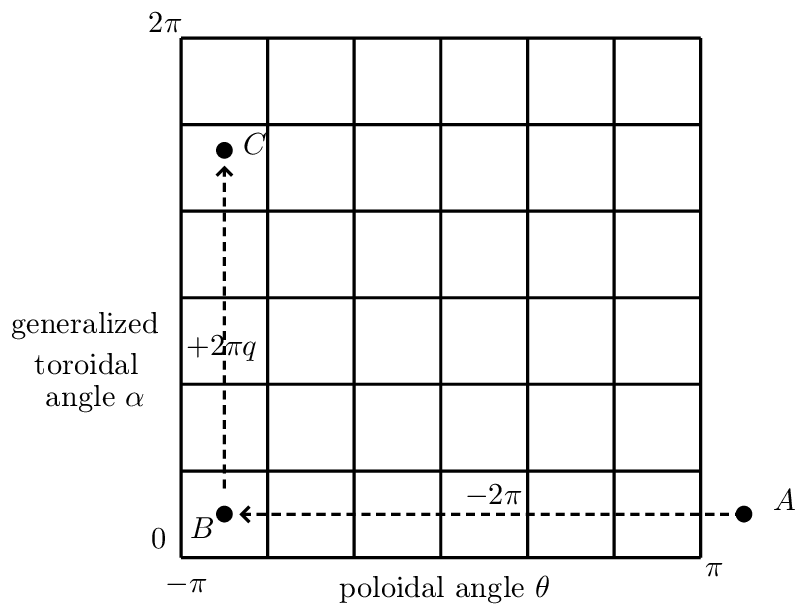
\includegraphics{/home/yj/theory/guiding_center_motion/figures/fig1/shift-1.eps}}
  \caption{\label{17-11-4-1}To keep the point at the same spatial location
  when shifting $\theta$ by $- 2 \pi$, $\alpha$ should be shifted by $+ 2 \pi
  q$. Here $A$ and $C$ correspond to the same spatial location, but $B$ is at
  a different location.}
\end{figure}

\

\

\begin{figure}[h]
  \resizebox{12cm}{!}{\includegraphics{/home/yj/project_new/fig_lorentz/fig2018-2-3e1/f.eps}}
  \caption{\label{18-2-4-p1}Temporal evolution of $(\psi, \theta, \alpha)$ of
  a passing electron. The range of $\theta$ is chosen to be $[- \pi : \pi]$
  and the range of $\alpha$ and $\phi$ is $[0 : 2 \pi]$. When $\theta$ exeed
  the range, a $2 \pi$ shift is imposed, which generate the jump of $\theta$
  in (b) and also the corresponding jump of $\alpha$ in (c). Note that when a
  jump in $(\theta, \alpha)$ ocurs, no jump in $\phi$, which is what we
  expect, otherwise there must be something wrong. Also note that there are
  also jumps of $\phi$ shown in (c), which is due to $\phi$ exceeding the
  range $[0 : 2 \pi]$ and a $2 \pi$ shift being imposed and this jump has
  nothing to do with the jump in $\theta$ or $\alpha$ and usually occur at
  different time (one jump of $\phi$ is near the jump of $\alpha$, which is
  only a coincidence). Here $\phi$ is computed using $\phi = \alpha +
  \overline{\delta}$, where $\overline{\delta}$ is obtained by interpolating
  the 2D numerical table of $\overline{\delta} (\psi, \theta)$. DIID-D cyclone
  base case}
\end{figure}

\

(When $\alpha$ of a particle moves beyong the range $[0 : 2 \pi]$, one or
multiple $\pm 2 \pi$ shifts are imposed on $\alpha$ until $\alpha$ are within
$[0 : 2 \pi]$. Since, for fixed $\psi$ and $\theta$, the generalized toroidal
angle $\alpha$ is equivalent to the usual toroidal angle $\phi$. No
complication like the case of $\theta$ arises when doing the $\alpha$ shift.)

One way of avoiding the subtle $(\theta, \alpha)$ shift problem is to evolve
particles' $\phi$, instead of $\alpha$. In this case, we have


\begin{eqnarray}
  \frac{d \phi}{d \overline{t}} = \overline{\mathbf{v}}_d \cdot
  \overline{\nabla} \phi & = & \overline{v}_{\parallel}
  \frac{\overline{\mathbf{B}} + \frac{\overline{v_{\parallel}}}{2 \pi}
  \overline{\nabla} \times \mathbf{b}}{\overline{B} \left( 1 +
  \frac{\overline{v}_{\parallel}}{2 \pi \overline{B}} \mathbf{b} \cdot
  \overline{\nabla} \times \mathbf{b} \right)} \cdot \overline{\nabla} \phi +
  \frac{\overline{\mu}}{2 \pi \left( 1 + \frac{\overline{v}_{\parallel}}{2 \pi
  \overline{B}} \mathbf{b} \cdot \overline{\nabla} \times \mathbf{b} \right)}
  \frac{1}{\overline{B}^2} \overline{\mathbf{B}} \times \overline{\nabla}
  \overline{B} \cdot \overline{\nabla} \phi, 
\end{eqnarray}
After geting $\phi$, we use $\alpha = \phi - \overline{\delta} (\psi, \theta)$
to get particles' $\alpha$, where $\overline{\delta}$ is obtained by
interpolating the numerical table in $(\psi, \theta)$ plane. I have tested the
two ways of computing evolution of $\alpha$, which indicates their results
agree with each other. In the final codes, I use the $(\theta, \alpha)$ shift
method, because this methods involve less interpolation and thus more
efficient.

\subsubsection{Benchmarking cases}

To verify code implementation, two methods are used to compute the
guiding-center orbits. The first method uses the cylindrical coordinates and
then interpolate the orbits into magnetic coordinates using pre-computed
mapping table between the cylindrical and magnetic coordinates. The second
method directly uses the magnetic coordinates in pushing the orbits. The
following figures compare the results obtained by these two methods, which
indicates they agree with each other. This provdies confidence on the
correctness of the numerical implementation.

\begin{figure}[h]
  \resizebox{12cm}{!}{\includegraphics{/home/yj/project_new/fig_lorentz/fig2018-2-3e1/figb/f.eps}}
  \caption{\label{18-2-4-e1}Comparison between the temporal evolution of
  $(\psi, \theta, \alpha)$ of a passing electron computed by two methods: the
  blue lines are the results computed directly in $(\psi, \theta, \alpha)$
  field-line-following coordinates, the red lines are results computed in
  cylindrical coordinates and then interpolated to the field-line-following
  coordinates. There is sysmetical discrepancy between $\psi$ computed by the
  two methods. The results are actually very close to each other and the
  differebce becomes obvious because the variation of $\psi$ is very small for
  a passing electron.
  The results of $\alpha$ from the two methods also agree with each other.
  The discrepancy near $t \Omega_i = 400$ is due to that $\alpha$ is close to
  $2 \pi$, and one result becomes zero, which is equivalent to $2 \pi$.
  equilibrium is the DIID-D cyclone base case}
\end{figure}

\

\

\

\begin{figure}[h]
  \includegraphics{/home/yj/project_new/lorentz_ions/figures/fig2e/p.eps}\includegraphics{/home/yj/project_new/lorentz_ions/figures/fig2/p.eps}
  \caption{Left: orbit on poloidal plane. Right: $\alpha$ is defined by
  $\alpha = \phi - \int_0^{\theta} \hat{q} d \theta,$ where $\phi$ is the
  usual cylindrical toroidal angle.}
\end{figure}

\

\

\

\begin{figure}[h]
  \
  
  \includegraphics{/home/yj/project_new/lorentz_ions/figures/fig2c/p.eps}\includegraphics{/home/yj/project_new/lorentz_ions/figures/fig2f/p.eps}
  
  \includegraphics{/home/yj/project_new/lorentz_ions/figures/fig2b/p.eps}\includegraphics{/home/yj/project_new/lorentz_ions/figures/fig2d/p.eps}
  \caption{The evolutions of the poloidal angles $\theta$ and generalized
  toroidal anglecal $\alpha$ culated by the two methods agree with each
  other.\quad$r = \sqrt{\frac{\Psi - \Psi_0}{\Psi_b - \Psi_0}}$}
\end{figure}

\

\subsection{Equations of guiding-center motion in cylindrical coordinates}

In this section, all quantities are in the normalized form given in Sec.
\ref{5-17-1}. For notational simplicity, the overbars of the notation are
ommitted. In cylindrical coordinates $(R, \phi, Z)$, the location vector is
written as $\mathbf{X}= R \hat{\mathbf{e}}_R + Z \hat{\mathbf{e}}_Z$. Using
this, we obtain
\begin{equation}
  \frac{d\mathbf{X}}{d t} = \frac{d R}{d t} \hat{\mathbf{e}}_R + R \frac{d
  \phi}{d t} \hat{\mathbf{e}}_{\phi} + \frac{d Z}{d t} \hat{\mathbf{e}}_Z
\end{equation}
Substituting this into Eq. (\ref{5-15-p2}) gives
\begin{equation}
  \frac{d R}{d t} \hat{\mathbf{e}}_R + R \frac{d \phi}{d t}
  \hat{\mathbf{e}}_{\phi} + \frac{d Z}{d t} \hat{\mathbf{e}}_Z =
  \frac{\mathbf{B}^{\star}}{B^{\star}_{\parallel}} v_{\parallel} +
  \frac{\mu}{2 \pi B B^{\star}} \mathbf{B} \times \nabla B + \frac{1}{B
  B^{\star}_{\parallel}} \mathbf{E} \times \mathbf{B},
\end{equation}
from which we obtain the following component equations:
\begin{equation}
  \frac{d R}{d t} = \left[ \frac{\mathbf{B}^{\star}}{B^{\star}_{\parallel}}
  v_{\parallel} + \frac{\mu}{2 \pi B B^{\star}_{\parallel}} \mathbf{B} \times
  \nabla B + \frac{1}{B B_{\parallel}^{\star}} \mathbf{E} \times \mathbf{B}
  \right] \cdot \hat{\mathbf{e}}_R
\end{equation}
\begin{equation}
  \frac{d Z}{d t} = \left[ \frac{\mathbf{B}^{\star}}{B^{\star}_{\parallel}}
  v_{\parallel} + \frac{\mu}{2 \pi B B^{\star}_{\parallel}} \mathbf{B} \times
  \nabla B + \frac{1}{B B_{\parallel}^{\star}} \mathbf{E} \times \mathbf{B}
  \right] \cdot \hat{\mathbf{e}}_Z,
\end{equation}
\begin{equation}
  \frac{d \phi}{d t} = \frac{1}{R} \left[
  \frac{\mathbf{B}^{\star}}{B^{\star}_{\parallel}} v_{\parallel} +
  \frac{\mu}{2 \pi B B^{\star}_{\parallel}} \mathbf{B} \times \nabla B +
  \frac{1}{B B_{\parallel}^{\star}} \mathbf{E} \times \mathbf{B} \right] \cdot
  \hat{\mathbf{e}}_{\phi},
\end{equation}
In the cylindrical coordinates, the terms $\nabla \times \mathbf{b}$,
$\mathbf{b} \cdot \nabla \times \mathbf{b}$, and $\mathbf{B} \times \nabla B$
can be written, respectively, as
\begin{eqnarray}
  \nabla \times \mathbf{b} & = & \left( \frac{1}{R}  \frac{\partial
  b_Z}{\partial \phi} - \frac{\partial b_{\phi}}{\partial z} \right) \hat{e}_R
  + \left(  \frac{\partial b_R}{\partial Z} - \frac{\partial b_Z}{\partial R}
  \right) \hat{e}_{\phi} + \left( \frac{1}{R}  \frac{\partial (R
  b_{\phi})}{\partial R} - \frac{1}{R}  \frac{\partial b_R}{\partial \phi}
  \right) \hat{e}_Z 
\end{eqnarray}
\begin{equation}
  \mathbf{b} \cdot \nabla \times \mathbf{b}= b_R \left( \frac{1}{R} 
  \frac{\partial b_Z}{\partial \phi} - \frac{\partial b_{\phi}}{\partial z}
  \right) + b_{\phi} \left(  \frac{\partial b_R}{\partial Z} - \frac{\partial
  b_Z}{\partial R} \right) + b_Z \left( \frac{1}{R}  \frac{\partial (R
  b_{\phi})}{\partial R} - \frac{1}{R}  \frac{\partial b_R}{\partial \phi}
  \right) .
\end{equation}
\begin{equation}
  \mathbf{B} \times \nabla B = \left|\begin{array}{ccc}
    \hat{e}_R & \hat{e}_{\phi} & \hat{e}_Z\\
    B_R & B_{\phi} & B_Z\\
    \frac{\partial B}{\partial R} & \frac{1}{R}  \frac{\partial B}{\partial
    \phi} & \frac{\partial B}{\partial Z}
  \end{array}\right|
\end{equation}
Using $b_R = \frac{B_R}{B}$, $b_Z = \frac{B_Z}{B}$, and $b_{\phi} =
\frac{B_{\phi}}{B}$, we obtain
\begin{equation}
  \left\{ \begin{array}{l}
    \frac{\partial b_R}{\partial R} = \frac{\frac{\partial B_R}{\partial R} B
    - \frac{\partial B}{\partial R} B_R}{B^2}\\
    \frac{\partial b_R}{\partial Z} = \frac{\frac{\partial B_R}{\partial Z} B
    - \frac{\partial B}{\partial Z} B_R}{B^2}\\
    \frac{\partial b_R}{\partial \phi} = \frac{\frac{\partial B_R}{\partial
    \phi} B - \frac{\partial B}{\partial \phi} B_R}{B^2}
  \end{array} \qquad \right\{ \begin{array}{l}
    \frac{\partial b_Z}{\partial R} = \frac{\frac{\partial B_Z}{\partial R} B
    - \frac{\partial B}{\partial R} B_Z}{B^2}\\
    \frac{\partial b_Z}{\partial Z} = \frac{\frac{\partial B_Z}{\partial Z} B
    - \frac{\partial B}{\partial Z} B_Z}{B^2}\\
    \frac{\partial b_Z}{\partial \phi} = \frac{\frac{\partial B_Z}{\partial
    \phi} B - \frac{\partial B}{\partial \phi} B_Z}{B^2}
  \end{array} \quad \left\{ \begin{array}{l}
    \frac{\partial b_{\phi}}{\partial R} = \frac{\frac{\partial
    B_{\phi}}{\partial R} B - \frac{\partial B}{\partial R} B_{\phi}}{B^2}\\
    \frac{\partial b_{\phi}}{\partial Z} = \frac{\frac{\partial
    B_{\phi}}{\partial Z} B - \frac{\partial B}{\partial Z} B_{\phi}}{B^2}\\
    \frac{\partial b_{\phi}}{\partial \phi} = \frac{\frac{\partial
    B_{\phi}}{\partial \phi} B - \frac{\partial B}{\partial \phi}
    B_{\phi}}{B^2}
  \end{array} \right.
\end{equation}
The equation for $v_{\parallel}$ is given by
\begin{equation}
  \frac{d v_{\parallel}}{d t} = - \mu
  \frac{\mathbf{B}^{\star}}{B^{\star}_{\parallel}} \cdot \nabla B + 2 \pi
  \frac{\mathbf{B}^{\star}}{B^{\star}_{\parallel}} \cdot \mathbf{E}.
\end{equation}
The first term on the left-hand-side of the above equation is written
\begin{equation}
  \frac{\mathbf{B}^{\star}}{B^{\star}_{\parallel}} \cdot \nabla B =
  \frac{B^{\star}_R}{B^{\star}_{\parallel}}  \frac{\partial B}{\partial R} +
  \frac{B^{\star}_{\phi}}{B^{\star}_{\parallel}}  \frac{1}{R}  \frac{\partial
  B}{\partial \phi} + \frac{B^{\star}_Z}{B^{\star}_{\parallel}} 
  \frac{\partial B}{\partial Z}
\end{equation}
\begin{equation}
  B^{\star}_R = B_R + \frac{v_{\parallel}}{2 \pi} \left( \frac{1}{R} 
  \frac{\partial b_Z}{\partial \phi} - \frac{\partial b_{\phi}}{\partial z}
  \right)
\end{equation}

\begin{equation}
  B^{\star}_Z = B_Z + \frac{v_{\parallel}}{2 \pi} \left( \frac{1}{R} 
  \frac{\partial (R b_{\phi})}{\partial R} - \frac{1}{R}  \frac{\partial
  b_R}{\partial \phi} \right)
\end{equation}
\begin{equation}
  B^{\star}_{\phi} = B_{\phi} + \frac{v_{\parallel}}{2 \pi} \left( 
  \frac{\partial b_R}{\partial Z} - \frac{\partial b_Z}{\partial R} \right)
\end{equation}


\subsection{Equilibrium magnetic field in tokamak}

The tokamak equilbrium magnetic field can be written
\begin{equation}
  \label{10-28-e1} \mathbf{B}= \nabla \Psi \times \nabla \phi + g (\Psi)
  \nabla \phi .
\end{equation}
In my code, the values of the two free functions, $\Psi = \Psi (R, Z)$ and $g
(\Psi)$, which sepcify the magnetic field, is read from the output file
``G-eqdsk-file'' of EFIT code. Using Eq. (\ref{10-28-e1}), the axisymmetric
equilibrium magnetic field can be written as
\begin{equation}
  B_R = - \frac{1}{R}  \frac{\partial \Psi}{\partial Z},
\end{equation}
\begin{equation}
  B_Z = \frac{1}{R}  \frac{\partial \Psi}{\partial R},
\end{equation}
\begin{equation}
  B_{\phi} = \frac{g (\Psi)}{R} .
\end{equation}
The partial derivative of the component of the magnetic field is written as
\begin{equation}
  \frac{\partial B_R}{\partial R} = \frac{1}{R^2}  \frac{\partial
  \Psi}{\partial Z} - \frac{1}{R} \frac{\partial^2 \Psi}{\partial Z \partial
  R}
\end{equation}
\begin{equation}
  \frac{\partial B_R}{\partial Z} = - \frac{1}{R}  \frac{\partial^2
  \Psi}{\partial Z^2}
\end{equation}
\begin{equation}
  \frac{\partial B_Z}{\partial R} = - \frac{1}{R^2}  \frac{\partial
  \Psi}{\partial R} + \frac{1}{R} \frac{\partial^2 \Psi}{\partial R^2}
\end{equation}
\begin{equation}
  \frac{\partial B_Z}{\partial Z} = \frac{1}{R}  \frac{\partial^2
  \Psi}{\partial R \partial Z}
\end{equation}

\begin{equation}
  \frac{\partial B_{\phi}}{\partial R} = - \frac{1}{R^2} g (\Psi) +
  \frac{1}{R} g' (\Psi) \frac{\partial \Psi}{\partial R}
\end{equation}
\begin{equation}
  \frac{\partial B_{\phi}}{\partial Z} = \frac{1}{R} g' (\Psi) \frac{\partial
  \Psi}{\partial Z}
\end{equation}



\begin{equation}
  \Rightarrow B = \frac{1}{R} \sqrt{\left(  \frac{\partial \Psi}{\partial R}
  \right)^2 + \left(  \frac{\partial \Psi}{\partial Z} \right)^2 + g^2}
\end{equation}

\begin{eqnarray}
  \frac{\partial B}{\partial R} & = & - \frac{1}{R^2} B R + \frac{1}{R} 
  \frac{1}{2}  \frac{1}{B R} \left( 2 \frac{\partial \Psi}{\partial R} 
  \frac{\partial^2 \Psi}{\partial R^2} + 2 \frac{\partial \Psi}{\partial Z} 
  \frac{\partial^2 \Psi}{\partial Z \partial R} + 2 g \frac{\partial
  g}{\partial R} \right) \nonumber\\
  & = & - \frac{B}{R} + \frac{1}{B R^2} \left( \frac{\partial \Psi}{\partial
  R}  \frac{\partial^2 \Psi}{\partial R^2} + \frac{\partial \Psi}{\partial Z} 
  \frac{\partial^2 \Psi}{\partial Z \partial R} + g \frac{\partial g}{\partial
  R} \right) 
\end{eqnarray}

\begin{eqnarray}
  \frac{\partial B}{\partial Z} & = & \frac{1}{R} \frac{1}{2}  \frac{1}{B R}
  \left( 2 \frac{\partial \Psi}{\partial R}  \frac{\partial^2 \Psi}{\partial R
  \partial Z} + 2 \frac{\partial \Psi}{\partial Z}  \frac{\partial^2
  \Psi}{\partial Z^2} + 2 g \frac{\partial g}{\partial Z} \right) \nonumber\\
  & = &  \frac{1}{B R^2} \left( \frac{\partial \Psi}{\partial R} 
  \frac{\partial^2 \Psi}{\partial R \partial Z} + \frac{\partial
  \Psi}{\partial Z}  \frac{\partial^2 \Psi}{\partial Z^2} + g \frac{\partial
  g}{\partial Z} \right) 
\end{eqnarray}


In my numerical code, the numerical data of the poloidal flux function $\Psi
(R, Z)$ and toroidal field function $g (\Psi)$ are read in from the output
G-eqdsk file of the EFIT code. Then all the partial derivatives are calculated
by using central finite-difference. Then the linear interpolation is used to
evaluate the various quantities that are needed at the instantenous location
of guiding-centers to push the orbits.

\subsubsection{Solov{\'e}v equilibrium}

When I began to write the guiding center orbit code, in order to avoid the
numerical interpolating, I use Solovev's analytic equilibrium. (The latest
version of my code constructs magnetic field by reading the output G-eqdsk
file of the EFIT code and thus can treat general tokamak magnetic field.) The
Solov{\'e}v equilibrium is an analytic equilibrium in which the poloidal flux
function $\Psi$ is given by
\begin{equation}
  \label{11-21-p1} \Psi = \frac{B_0}{2 R_0^2 \kappa_0 q_0} \left[ R^2 Z^2 +
  \frac{\kappa_0^2}{4} (R^2 - R_0^2)^2 \right],
\end{equation}
where $B_0$, $R_0$, $\kappa_0$, $q_0$ are constant parameters. Using Eq.
(\ref{11-21-p1}), the partial derivatives are written as
\begin{equation}
  \frac{\partial \Psi}{\partial R} = \frac{B_0}{2 R_0^2 \kappa_0 q_0} [2 R Z^2
  + \kappa_0^2 (R^2 - R_0^2) R], \frac{\partial \Psi}{\partial Z} =
  \frac{B_0}{R_0^2 \kappa_0 q_0} R^2 Z.
\end{equation}

\begin{equation}
  \frac{\partial^2 \Psi}{\partial R^2} = \frac{B_0}{2 R_0^2 \kappa_0 q_0} [2
  Z^2 + \kappa_0^2 (3 R^2 - R_0^2)]
\end{equation}
\begin{equation}
  \frac{\partial^2 \Psi}{\partial Z^2} = \frac{B_0}{R_0^2 \kappa_0 q_0} R^2,
  \frac{\partial^2 \Psi}{\partial R \partial Z} = \frac{2 B_0}{R_0^2 \kappa_0
  q_0} R Z
\end{equation}
\begin{equation}
  \ 
\end{equation}
The toroidal field function $g$ is a constant function, $g = c_g R_0 B_0$,
where $c_g$ is a dimensionless constant.

\subsection{Initial conditions}

The initial conditions of the particle are given by specifying the initial
location $(R, \phi, Z)$, initial parallel velocity $v_{\parallel}$, and the
magnetic moment $\mu$ (which acts as a parameter since $\mu$ is exactly
conserved). In some cases, we prefer to specify the initial velocity in terms
of the initial kinetic energy $\varepsilon$ and the initial pitch angle
$\theta$ (the include angle between velocity and the local magnetic field).
The relation between $(\varepsilon, \theta)$ and $(v_{\parallel}, \mu)$ is
given by
\begin{equation}
  \mu = \frac{m v_{\perp}^2}{2 B} = \frac{m v^2}{2 B} \sin^2 \theta =
  \frac{\varepsilon}{B} \sin^2 \theta,
\end{equation}
and
\begin{equation}
  v_{\parallel} = v \sin \theta = \sqrt{\frac{2 \varepsilon}{m}} \cos \theta .
\end{equation}
The relation between $(\varepsilon, \theta)$ and the normalized quantities
$(\overline{\mu}, \overline{v}_{\parallel})$ is given by
\begin{equation}
  \overline{\mu} = \frac{\mu}{\mu_n} = \frac{\varepsilon}{B} \sin^2 \theta
  \frac{1}{m v_n^2 / B_n} = \frac{\varepsilon}{m v_n^2 \overline{B}} \sin^2
  \theta,
\end{equation}
and
\begin{equation}
  \overline{v}_{\parallel} = \sqrt{\frac{2 \varepsilon}{m v_n^2}} \cos \theta
  .
\end{equation}


\

\

\

------


\[ 2 (\varepsilon - B \mu) - \frac{1}{m} (P_{\phi} - Z e \Psi)^2 \left(
   \frac{B}{g} \right)^2 = 0 \]
\[ 2 \left( 1 - \frac{B}{B_0} \lambda \right) - (P_{\phi} - Z e \Psi)^2 \left(
   \frac{B}{g} \right)^2 \frac{1}{m \varepsilon} = 0, \]
where $\lambda = B_0 \mu / \varepsilon$

\

-------

\section{Benchmark of the code}

There are three constants of motion for the guiding center motion, namely, the
canonical toroidal angular momentum $P_{\phi}$, the magnetic moment $\mu$, and
the total kinetic energey $\varepsilon$. Examining how well the kinetic energy
$\varepsilon$ and the toroidal angular momentum $P_{\phi} $are conserved
provides a way to evaluate the accuracy of the numerical code. The kinetic
energy $\varepsilon$ and toroidal angular momentum $P_{\phi}$ are defined by
\begin{equation}
  \varepsilon = \frac{1}{2} m v^2 = \frac{1}{2} m v_{\parallel}^2 + B \mu
\end{equation}
\begin{equation}
  \label{9-28-1} P_{\phi} = m \frac{g (\Psi) }{B} v_{\parallel} + Z e \Psi,
\end{equation}
Define $\varepsilon_n = m v_n^2$ and $P_{\phi n} = Z e B_n L^2_n$, then the
normalized forms of $\varepsilon$ and $P_{\phi}$ are written as
\begin{equation}
  \overline{\varepsilon} \equiv \frac{\varepsilon}{m v_n^2} = \frac{1}{2}
  \overline{v}_{\parallel}^2 + \overline{\mu} \overline{B}
\end{equation}
\begin{eqnarray}
  \overline{P}_{\phi} & \equiv & \frac{P_{\phi}}{P_{\phi n}} \nonumber\\
  & = & \frac{1}{2 \pi}  \overline{g}  \frac{\overline{v}_{\parallel}
  }{\overline{B}} + \overline{\Psi} 
\end{eqnarray}
Figure \ref{8-10-e1} plots the time evolution of the kinetic energy
$\overline{\varepsilon}$ and toroidal angular momentum $\overline{P}_{\phi}$
for an energetic ion in EAST magnetic configuration. The results shows that
$\overline{\varepsilon}$ and $\overline{P}_{\phi}$ are conserved to acceptable
accuracy for a long time (100 poloidal periods of the orbit).

\begin{figure}[h]
  \includegraphics{/home/yj/project_new/guiding_center_motion/fig31b/p.eps}\includegraphics{/home/yj/project_new/guiding_center_motion/fig31/p.eps}\includegraphics{/home/yj/project_new/guiding_center_motion/fig31c/p.eps}
  \caption{\label{8-10-e1}Time evolution of the kinetic energy
  $\overline{\varepsilon}$ (a) and toroidal angular momentum
  $\overline{P}_{\phi}$ (b) for a Deuteron of $20 \tmop{keV}$ launched at the
  low-field-side midplane $(R_{\tmop{ini}} = 2.15 m, Z_{\tmop{ini}} = 0 m)$
  with pitch angle $\theta = 75^{\circ}$. The results shows that
  $\overline{\varepsilon}$ and $\overline{P}_{\phi}$ are conserved to
  acceptable accuracy ($\overline{\varepsilon}_k$ decreased by $1.8 \times
  10^{- 5}$ and $\bar{P}_{\phi}$ by $3.2 \times 10^{- 4}$ during the time of
  100 poloidal periods). The corresponding poloidal orbit is plotted in (c).
  Fourth-order Runge-Kutta time advancing scheme is used in integrating the
  orbit with a time step of $1 / 183$ poloidal period. The magnetic
  equilibrium is from EAST discharge \#62585@2.8s (gfile provided by
  ZhengZheng).}
\end{figure}

\subsection{Trapped and circulating particles}\label{15-9-25-1}

An approximate condition determining whether a particle is trapped or
circulating can be obtained by using the conservation of magnetic moment and
kinetic energy, and assuming the guiding center orbit is along the magnetic
field line (zero-width orbit approximation, which is a proper approximation
for low-energy particles whose orbit width is small, as is shown in Fig.
\ref{16-7-12-1}).

\begin{figure}[h]
  \includegraphics{/home/yj/project_new/guiding_center_motion/fig32/p.eps}
  \caption{\label{16-7-12-1}The magnetic field becomes stronger when a
  particle move inboard (toward smaller $R$). Due to the conservation of
  kinetic enery and magnetic moment, the magnitude of the paralell velocity
  decrease when a particle moves inboard. Also shown is the poloidal
  projection of guiding-center orbit for a particle of energy $2 \tmop{keV}$
  launched at the low-field-side midplane $(R = 2.25 m, Z = 0 m)$ with a pitch
  angle $\theta = 115^{\circ}$.}
\end{figure}

In this approximation, the orbit remains on a magnetic surface. The critical
condition for a particle to be trapped or circulating is given by
\begin{equation}
  \label{4-24-e3} \frac{m v_{I \perp}^2}{2 B_I} = \frac{m v^2}{2 B_{\max}},
\end{equation}
where $v_{I \perp}$ is the initial perpendicular (to the magnetic field)
velocity of the particle, $B_I$ is the strength of the magnetic field at the
initial location of the particle, $B_{\max}$ is the maximum value of the
magentic field on the same magnetic surface where the particle moves. Equation
(\ref{4-24-e3}) can be written
\begin{equation}
  \label{15-9-25-2} \sin^2 \theta_I = \frac{B_I}{B_{\max}},
\end{equation}
where $\theta_I = \arccos (v_{I \perp} / v)$ is the initial pitch angle of
velocity with respect to the local magnetic field. It is obvious that
particles with $\sin^2 \theta_I > B_I / B_{\max}$ can not reach the point of
the maximum magnetic field of the same magnetic surface and thus they are
trapped particles. Otherwise, they are circulating particles. In velocity
space $(v_{\parallel}, v_{\perp})$, the trapped and circulating region are
shown in Fig. \ref{2-1-2}.

\

\begin{figure}[h]
  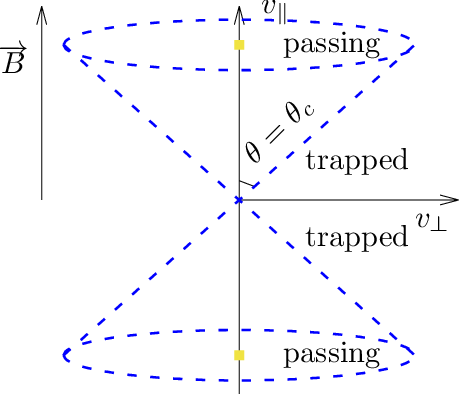
\includegraphics{/home/yj/theory/figures/passing_trapped/p_processed.eps}
  \caption{\label{2-1-2}Passing and trapped regions in the phase-space
  $(v_{\parallel}, v_{\perp})$. The boundary between passing and trapped
  region is given by $\theta_I = \theta_{\tmop{tr}}$, where
  $\theta_{\tmop{tr}}$ is determined by $\sin^2 \theta_{\tmop{tr}} = B_I /
  B_{\max}$; $B_I$ and $B_{\max}$ are respectively the local (at the initial
  location of the particle) and maximal value of the magnetic field on one
  magnetic surface.}
\end{figure}

Note that the trapped-circulating boundary given in Fig. \ref{2-1-2} is
determined based on the assumption that the guiding center motion does not
deviate from a magnetic surface. However, the actual guiding center orbit does
not remain on the same magnetic surface, so the above result can be wrong when
applied to some particles. An example is given in Fig. \ref{6-12-a8}, where
the numerical results show that the particle is actually trapped but the
approximate condition indicate that the particle is circulating.

\

\begin{figure}[h]
  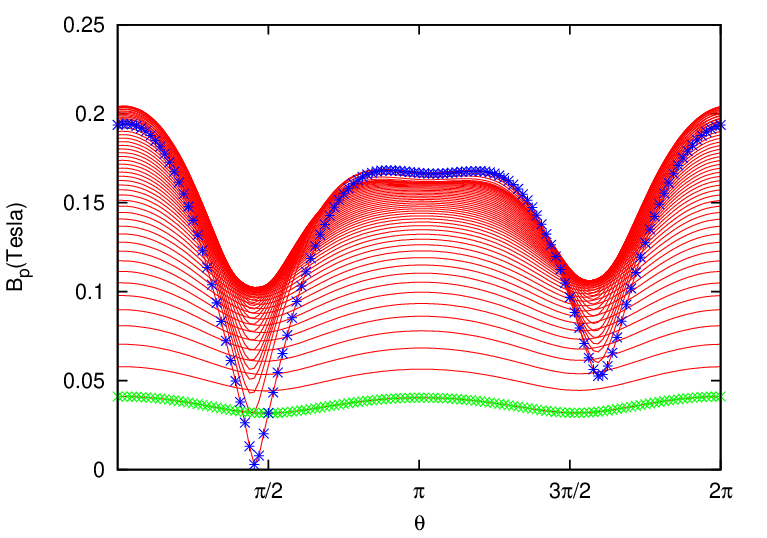
\includegraphics{/home/yj/project_new/guiding_center_motion/fig8/p3.eps}
  \caption{\label{6-12-a8}Numerical orbit of a particle on the poloidal plane,
  which show that the particle is trapped. However, the particle would be
  considered to be circulating if we used the approximate condition given in
  Fig. \ref{2-1-2}. It is easy to understand why the approximate condition
  breaks down for this case: the orbit derivates from the original flux
  surface (i.e., the zero-width orbit)to the stronger field region.}
\end{figure}

In terms of $(w, \mu)$ coordinates, where $w$ is the kinetic energy, the
trapped regions and the passing regions of pahse space are shown in Fig.
\ref{10-31-p1}.

\begin{figure}[h]
  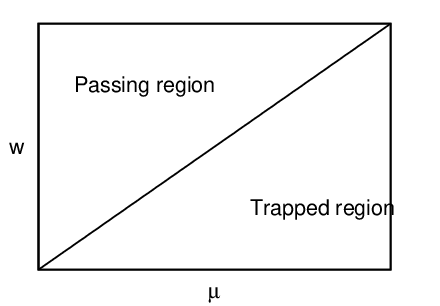
\includegraphics{/home/yj/theory/figures/passing-trapped.eps}
  \caption{\label{10-31-p1}The passing and the trapped regions of phase space
  $(w, \mu)$. The boundary between passing and trapped region is given by $w =
  \mu B_{\max}$, where $B_{\max}$ is the maximum value of magnetic field on
  the same magnetic surface where the particle moves.}
\end{figure}

\subsection{Analytical estimation of bounce frequency of deeply trapped
particles}

The time evolution of the paralell velocity of a guiding center is given by
Eq. (\ref{16-7-4-7}), i.e.,
\begin{equation}
  \frac{d v_{\parallel}}{d t} = - \frac{\mu}{m} 
  \frac{\mathbf{B}^{\star}}{B^{\star}_{\parallel}} \cdot \nabla B,
\end{equation}
which can be approximately written as
\[ \frac{d v_{\parallel}}{d t} = - \frac{\mu}{m} \mathbf{b} \cdot \nabla B, \]
which can be further written as
\begin{equation}
  \label{16-7-4-3} \frac{d^2 l}{d t^2} = - \frac{v_{\perp}^2}{2 B} \frac{d
  B}{d l}
\end{equation}
where $d l$ is the arc lengh along the magnetic field. In a large aspect ratio
tokamak with circular flux surfaces, the magnetic field can be written
approximatedly as
\begin{equation}
  \label{16-7-4-2} B = \frac{B_0}{1 + (r / R_0) \cos \theta},
\end{equation}
The equation of magnetic field is written
\begin{equation}
  \frac{B_{\theta}}{B} = \frac{d l_p}{d l} = \frac{r d \theta}{d l},
\end{equation}
which can be written
\begin{equation}
  \label{16-7-4-1} d l = \frac{B}{B_{\theta}} r d \theta
\end{equation}
Using Eqs. (\ref{16-7-4-1}) and (\ref{16-7-4-2}), the paralel derivative of
the magnetic field is written as
\begin{equation}
  \frac{d B}{d l} = \frac{B_{\theta}}{r B}  \frac{d B}{d \theta} =
  \frac{B_{\theta}}{r B}  \frac{B_0}{[1 + (r / R_0) \cos \theta]^2} 
  \frac{r}{R_0} \sin \theta,
\end{equation}
Using this, equation (\ref{16-7-4-3}) is written
\begin{equation}
  \frac{d^2 l}{d t^2} = - \frac{v_{\perp}^2}{2 B} \frac{B_{\theta}}{r B} 
  \frac{B_0}{[1 + (r / R_0) \cos \theta]^2}  \frac{r}{R_0} \sin \theta = -
  \frac{v_{\perp}^2}{2}  \frac{B_{\theta}}{B_0}  \frac{1}{R_0} \sin \theta
\end{equation}
Consider deeply trapped particles (particles are trapped in a very small
region near the low-field-side midplane), i.e., $\theta \approx 0$, then we
have $\sin \theta \approx \theta$. Using this, the above equation is written
as
\begin{equation}
  \label{16-7-4-6} \frac{d^2 l}{d t^2} \approx - \frac{v_{\perp}^2}{2} 
  \frac{B_{\theta}}{B_0}  \frac{1}{R_0} \theta
\end{equation}
Assume the orbit is along the magnetic field line (i.e. zero-width orbit
approximation), then the equation of magnetic field \ (\ref{16-7-4-1}) is also
satisfied by the orbit. In the linear approximation, we have $\theta \approx
B_{\theta} / (B r) l$. Using this in Eq. (\ref{16-7-4-6}), we obtain
\begin{equation}
  \frac{d^2 l}{d t^2} = - \frac{r v_{\perp}^2}{2 R_0}  \frac{B_{\theta}^2}{B^2
  r^2} l
\end{equation}
Using the definition of safety factor, $q = r B_0 / R_0 B_{\theta}$, the above
quation is written
\begin{equation}
  \label{16-7-4-5} \frac{d^2 l}{d t^2} = - \frac{v_{\perp}^2}{q^2 R_0^2} 
  \frac{r}{2 R_0} l
\end{equation}
Define
\begin{equation}
  \label{16-7-4-8} \omega_b = \frac{v_{\perp}}{q R_0}  \left( \frac{r}{2 R_0}
  \right)^{1 / 2},
\end{equation}
(for deeply trapped particles, the variation of $v_{\perp}$ during one
poloidal period is small, and thus can be considered constant, and thus
$\omega_b$ can also be considered constant), then Eq. (\ref{16-7-4-5}) is
written
\begin{equation}
  \label{16-7-5-1} \frac{d^2 l}{d t^2} = - \omega_b^2 l,
\end{equation}
which indicates that the motion of a deeply trapped particle is a harmonic
oscillation with an angular frequency $\omega_b$. Equations (\ref{16-7-4-8})
and (\ref{16-7-5-1}) agree with Eqs. (3.12.3) and (3.12.4) in Wesson's book
``Tokmaks''{\cite{wesson2004}}. I have test the accuracy of formula
(\ref{16-7-4-8}) by comparing it with the numerical results, which indicates
the formula can usually give a reasonable estimation of the bounce frequency
(for example, 28kHz is obtained numerically while the analytical formula gives
24kHz for a not very deeply trapped orbit)

\

\subsection{Methods of determining drift orbits}

If neglecting the magnetic drift, a guiding-center orbit is along a magnetic
field lines. Therefore there is no derivation from the magnetic surface where
a guiding center is initially located. Taking the magnetic drift into account,
a guiding-center orbit will deviate from the initial magnetic surface and the
orbit will have finite-width.

Whether a drift orbit is inside or outside of the local magnetic surface near
the midplane can be determined in the following way. First note that the
zero-order approximation of the guiding-center orbit (zero-width orbit) is
either parallel or anti-parallel to the local magnetic field, depending on the
sign of $v_{\parallel}$. Further note the direction of the magnetic drift
($\mathbf{B} \times \nabla B$ and curvature drift) is approximatedly vertical,
which can be either up or down, depending on the direction of the toroidal
magnetic field. Finally, by imposing the magnetic drift on the zero-width
orbit, we can determine whether the guiding center will drift inside or
outside of the local magnetic surface. Figures \ref{16-6-30-1}-\ref{16-6-30-3}
plots the drift orbits for all the possible combinitions of tokamak magnetic
configurations and particle initial conditions.

\

\begin{figure}[h]
  \includegraphics{/home/yj/project_new/guiding_center_motion/fig26/p.eps}\includegraphics{/home/yj/project_new/guiding_center_motion/fig26b/p.eps}
  
  \includegraphics{/home/yj/project_new/guiding_center_motion/fig26c/p.eps}\includegraphics{/home/yj/project_new/guiding_center_motion/fig26d/p.eps}
  \caption{\label{16-6-30-1}Projection of trapped orbits on the poloidal plane
  for various magnetic configurations. A Deuterium ion of $20 \tmop{keV}$ is
  launched from the low-field-side midplane $(R_{\tmop{initial}} = 2.15 m,
  Z_{\tmop{initial}} = 0 m)$ with pitch angle $\theta = 75^{\circ}
  (v_{\parallel} > 0)$ and $\theta = 105^{\circ} (v_{\parallel} < 0)$.
  $v_{\parallel} > 0$ implies that the zero-width orbit in the poloidal plane
  is along the direction of the poloidal magnetic field, which is in turn
  determined by the direction of the toroidal plasma current. The magnetic
  equilibrium is from EAST discharge \#62585@2.8s (gfile provided by
  ZhengZheng). The direction of toroidal plasma current, magnetic field, and
  the corresponding magnetic drift are indicated on the figures.}
\end{figure}

\

\

\begin{figure}[h]
  \includegraphics{/home/yj/project_new/guiding_center_motion/fig27/p.eps}\includegraphics{/home/yj/project_new/guiding_center_motion/fig27b/p.eps}
  
  \includegraphics{/home/yj/project_new/guiding_center_motion/fig27c/p.eps}\includegraphics{/home/yj/project_new/guiding_center_motion/fig27d/p.eps}
  \caption{\label{16-6-30-2}Projection of passing orbits on the poloidal plane
  for various magnetic configurations. A Deuterium ion of $20 \tmop{keV}$ is
  launched from the low-field-side midplane $(R_{\tmop{ini}} = 2.15 m,
  Z_{\tmop{ini}} = 0 m)$ with pitch angle $\theta = 50^{\circ} (v_{\parallel}
  > 0)$ and $\theta = 130^{\circ} (v_{\parallel} < 0)$. The magnetic
  equilibrium is from EAST discharge \#62585@2.8s (gfile provided by
  ZhengZheng). The direction of plasma current, magnetic field, and the
  corresponding magnetic drift are indicated on the figures.}
\end{figure}

\

\

\begin{figure}[h]
  \includegraphics{/home/yj/project_new/guiding_center_motion/fig28/p.eps}\includegraphics{/home/yj/project_new/guiding_center_motion/fig28b/p.eps}
  
  \includegraphics{/home/yj/project_new/guiding_center_motion/fig28c/p.eps}\includegraphics{/home/yj/project_new/guiding_center_motion/fig28d/p.eps}
  \caption{\label{16-6-30-3}Projection of passing orbits on the poloidal plane
  for various magnetic configurations. A Deuterium ion of $20 \tmop{keV}$ is
  launched from the high-field-side midplane $(R_{\tmop{ini}} = 1.6452 m,
  Z_{\tmop{ini}} = 0 m)$ with pitch angle $\theta = 50^{\circ} (v_{\parallel}
  > 0)$ and $\theta = 130^{\circ} (v_{\parallel} < 0)$. The magnetic
  equilibrium is from EAST discharge \#62585@2.8s (gfile provided by
  ZhengZheng). The direction of plasma current, magnetic field, and the
  corresponding magnetic drift are indicated on the figures.}
\end{figure}

\

Examining the above results, it is ready to realize that reversing the
direction of the toroidal magnetic field does not change the projection of
orbits on the poloidal plane, i.e., the location and shape of the poloidal
orbits remain the same. However the direction of the poloidal motion is
changed from clockwise (anti-clockwise) to anti-clockwise (clockwise). (This
is obvious because $v_{\parallel}$ of a particle changes sign when the
toroidal field is reversed and thus the direction of the poloidal motion
changes).

Examining the above results, we can also find that, for particles launched
from low-field-side midplane, co-current partilces have their orbits inside
the magnetic surface at which the particle is iniitally located, and
counter-current particles have thier orbits outside of the magnetic surface.
For particles launched from the high-field-side midplane, the conclusion is
reversed, i.e., co-current partilces have their orbits outside the magnetic
surface where they are iniitally located, and counter-current particles have
thier orbits inside of the magnetic surface.

These conclusions have important implications for the neutral beam injection,
where orbits outside a reference magnetic surface are more likely to be lost
to the wall of the machine. If the neutral beam injection (NBI) is along the
same direction of the plasma current, it is called the co-current injection.
Otherwise it is called the counter-current injection. Using the above
conclusions, we know that, for co-current injection, ions ionized at the
low-field-side have better confinement compared with those ionized at the
high-field-side. For the counter-current injection, ions ionized at the
high-field-side have better confinement compared with those ionized at the
low-field-side. Whether the overall confinment of ions due to co-current
injection is better or worse than that of the counter-current injection
depends on the ratio of number of ions deposited at the low-field-side to that
deposited at the high-field side. For the shine-through loss to be small, most
neutral must ionize at the low-field-side (most neutrals ionizing at the the
high-field side usually means a very high shine-through loss fraction
(>50\%)). Therefore, under the assumption that most neutral beam particles are
ionized on the low-field-side, it is right to say that co-curent injection is
better than counter-current injection.

\

Figure \ref{16-7-5-e1} and \ref{16-7-5-e2} compares the poloidal orbits of
energetic Deuterium particles ionized at the low-field-side midplane due to
co-current and counter-current injection. The results indicate again that the
counter-injected particles ionized at the low-field-side midplane are easy to
be lost from the plasma because their orbits are outside the flux surface
where they are ionized, and thus are more likely to touch the first wall.

\begin{figure}[h]
  \includegraphics{/home/yj/project_new/read_gfile/fig162/p.eps}
  \caption{\label{16-7-5-e1}Poloidal orbits of Deuterium particles of $50
  \tmop{keV}$ ionized at the low-field-side midplane $(R = 2.25 m, Z = 0 m)$
  with a birth pitch angle $\theta = 125^{\circ}$ (red), $\theta =
  105^{\circ}$ (blue), $\theta = 75^{\circ}$ (green), and $\theta =
  65^{\circ}$ (violet). Pitch angle $\theta$ is the included angle between the
  magnetic field and the velocity of particles. Since the magnetic field and
  the plasma current are in the same direction for this case, $\theta >
  90^{\circ}$ means counter-current injection and $\theta < 90^{\circ}$ means
  co-current injection. The counter-injected particles are easy to be lost
  from the plasma because their orbits are outside the flux surface where they
  are ionized, and thus are more likely to touch the first wall. The magnetic
  equilibrium is for EAST discharge \#62585@2.8s, which is a upper single-null
  configuration (gfile provided by ZhengZheng).}
\end{figure}

\

\begin{figure}[h]
  \includegraphics{/home/yj/project_new/read_gfile/fig162b/p.eps}
  \caption{\label{16-7-5-e2}Poloidal orbits of Deuterium particles of $50
  \tmop{keV}$ ionized at the low-field-side midplane $(R = 2.25 m, Z = 0 m)$
  with a birth pitch angle $\theta = 125^{\circ}$ (blue), $\theta =
  105^{\circ}$ (red), $\theta = 75^{\circ}$ (violet), and $\theta =
  60^{\circ}$ (green). Since the magnetic field and the plasma current are in
  the opposite direction for this case, $\theta > 90^{\circ}$ means co-current
  injection and $\theta < 90^{\circ}$ means counter-current injection. The
  magnetic equilibrium is from EAST discharge \#62585@2.8s but with the
  direction of the toroidal magnetic field reversed.}
\end{figure}

\

\begin{figure}[h]
  \includegraphics{/home/yj/project_new/read_gfile/fig162c/p.eps}
  \caption{The resonant layer of $50 \tmop{MHz}$ electromagnetic wave with the
  third harmonic of ion cyclotron frequency on EAST tokamak. The toroidal
  magnetic field of EAST is approximately given by $B_{\phi} = 4.160 \times
  10^{- 4} I_s / R$, where $I_s$ is the current in a single turn of the TF
  coils, which in in the range from $8000 A$ to $10000 A$ for usual EAST
  discharges. The ion cyclotron angular frequency is given by $\omega_{c i} =
  B_{\varphi} e / m_i$ ($f_{c i} = \omega_{\tmop{ci}} / 2 \pi$). The small
  Dopper frequency shift $k_{\parallel} v_{\parallel}$ is not included in the
  estimation of the resonant layer.}
\end{figure}

\

\subsection{Toroidal procession}

Figure \ref{1-31-e1} plots the guiding centers orbits for particles launched
at the low-field-side of the midplane with different values of the pitch angle
$\theta$.

\begin{figure}[h]
  \includegraphics{/home/yj/project_new/guiding_center_motion/fig11/p.eps}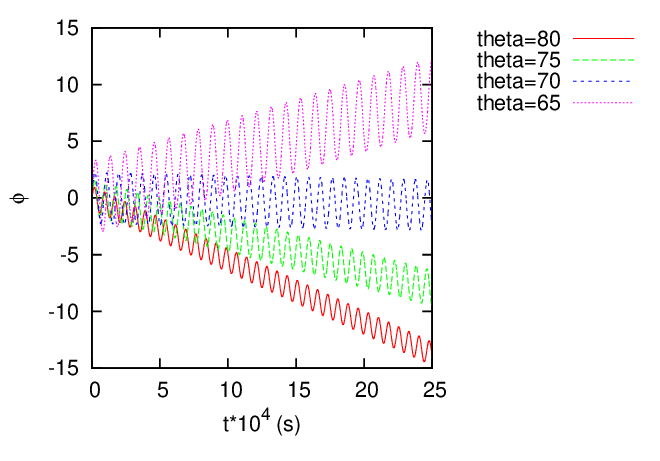
\includegraphics{/home/yj/project_new/guiding_center_motion/fig11/p2.eps}
  \caption{\label{1-31-e1}Left: projection of guiding center orbits of trapped
  particles on $(R, Z)$ plane. Right: Toroidal motion of guiding center of the
  trapped particles. All particles have the same kinetic energy $\varepsilon =
  10 \tmop{keV}$ and are launched from the low-field side midplane of the
  reference magnetic surface $(R = 2.1, Z = 0)$. The equilibrium is a Solovev
  equilibrium with $R_0 = 1.9 m, B_0 = 2.0 \tmop{Tesla}$, $\kappa_0 = 1.5$, $Z
  e_0 = 1.5$, $g = 3.8 \tmop{mT}$.}
\end{figure}

Figure \ref{1-31-e1} shows (1) the toroidal procesion of deeply trapped
particles is faster than that of the shallowly trapped particles and (2) the
direction of the toroidal precession of the particle with $\theta =
65^{\circ}$ is different from the others.

Procession angular frequency of a trapped particles (from Porcelli's slide):
\begin{equation}
  \omega_D = \frac{v^2}{2 \Omega_c R r} = \frac{E_k}{B Z e R r},
\end{equation}
where $E_k$ is the kinetic energy of the particle. Equation () indicates that
the procession frequency is proportional to the energy of the particle.
\begin{equation}
  \omega_D = \frac{v^2}{2 \Omega_c R r} = \frac{v^2}{2 \overline{B} \Omega_n
  \overline{R}  \overline{r} L_n^2} = \Omega_n \frac{\overline{v}^2}{8 \pi^2
  \overline{B}  \overline{R}  \overline{r}}
\end{equation}
Compared with the results given by the numerical code, the above results seems
to be roughly correct when the orbit is not near the magnetic axis.
\begin{equation}
  \overline{v}_{\perp}^2 = \frac{v_{\perp}^2}{v_n^2} = \frac{2 B \mu}{m v_n^2}
  = \overline{B} \frac{2 B_n \mu}{m v_n^2} = 2 \overline{B} \overline{\mu}
\end{equation}


\

\

\subsection{Radial drift --check!!}

\[ \frac{d \Psi}{d t} =\mathbf{V}_d \cdot \nabla \Psi = \frac{1}{\Omega}
   \mathbf{b} \times \left( \frac{\mu}{m} \nabla B + v_{\parallel}^2
   \mathbf{\kappa} \right) \cdot \nabla \Psi \]
\[ \frac{d \Psi}{d t} = \frac{1}{B \Omega} \mathbf{B} \times \left(
   \frac{\mu}{m} \nabla B + v_{\parallel}^2 \mathbf{\kappa} \right) \cdot
   \nabla \Psi \]
\[ \frac{d \Psi}{d t} = - \frac{1}{B \Omega} \mathbf{B} \times \nabla \Psi
   \cdot \left( \frac{\mu}{m} \nabla B + v_{\parallel}^2 \mathbf{\kappa}
   \right) \]
using
\[ \mathbf{B}= \nabla \Psi \times \nabla \phi + g \nabla \phi \]

\begin{equation}
  \label{16-6-24-1} \frac{d \Psi}{d t} = - \frac{1}{B \Omega} (\nabla \Psi
  \times \nabla \phi \times \nabla \Psi + g \nabla \phi \times \nabla \Psi)
  \cdot \left( \frac{\mu}{m} \nabla B + v_{\parallel}^2 \mathbf{\kappa}
  \right)
\end{equation}
Noting that both $\nabla B$ and $\mathbf{\kappa}$ are approximatedly along $-
\hat{\mathbf{R}}$ direction, which is perpendicular to $\nabla \phi$, Eq.
(\ref{16-6-24-1}) is written as


\[ \frac{d \Psi}{d t} = - \frac{1}{B \Omega} (g \nabla \phi \times \nabla
   \Psi) \cdot \left( \frac{\mu}{m} \nabla B + v_{\parallel}^2 \mathbf{\kappa}
   \right) \]
\[ \frac{d \Psi}{d t} = \frac{1}{B \Omega} g\mathbf{B}_p \cdot \left(
   \frac{\mu}{m} \nabla B + v_{\parallel}^2 \mathbf{\kappa} \right) \]


if
\[ \frac{d \Psi}{d t} (\Psi_{\tmop{lcfs}} - \Psi_{\tmop{axis}}) > 0, \]
then the drift from the local magnetic surface is outward, otherwise, the
drift is inward.
\[ \label{16-6-27-1} \frac{d \Psi}{d t} (\Psi_{\tmop{lcfs}} -
   \Psi_{\tmop{axis}}) = \frac{1}{B \Omega} g\mathbf{B}_p \cdot (-
   \hat{\mathbf{R}}) (\Psi_{\tmop{lcfs}} - \Psi_{\tmop{axis}}) \]
Examining the right-hand side of Eq. (\ref{16-6-27-1}), we find that
$\mathbf{B}_p$ and $(\Psi_{\tmop{lcfs}} - \Psi_{\tmop{axis}})$ change signs
simutaneouslly when the toroidal plasma current $I_{\phi}$ change sign, thus
the direction of $\mathbf{B}_p (\Psi_{\tmop{lcfs}} - \Psi_{\tmop{axis}})$ is
independent of the sign of $I_{\phi}$. Therefore the sign of the radial drift
is independent of the sign of $I_{\phi}$.

\subsection{Width of guiding center orbit}

The gyroradius of a particle is given by $r = m v / B Z e$, which can be
further written as
\begin{equation}
  \label{6-12-a1} r = \frac{\sqrt{2 m \varepsilon}}{B Z e},
\end{equation}
where $\varepsilon$ is the kinetic energy of the particle. For an electron
with the same kinetic energy of a ion, Eq. (\ref{6-12-a1}) indicates that the
gyroradius of the electron is smaller than that of the ion by the factor
$\sqrt{m_e / m_i}$. Now comes the question: Is the width of the guiding center
orbit of an electron with the same kinetic energy of a ion smaller than that
of the ion? Examine one of the constant of motion, $P_{\phi}$, which is given
by
\begin{equation}
  \frac{P_{\phi}}{Z e} = \frac{g (\Psi) }{\Omega} v_{\parallel} + \Psi,
\end{equation}
The function $g (\Psi) / \Omega$ is usually a weak function of $\Psi$, thus
can be asssumed to be a contant. The orbit width can be characterised by
$\Delta \Psi$, which is written
\begin{equation}
  \label{17-11-9-5} \Delta \Psi = - g \frac{\Delta v_{\parallel}}{\Omega} = -
  g \frac{m \Delta v_{\parallel}}{B Z e},
\end{equation}
where $\Delta v_{\parallel}$ is the variation range of $v_{\parallel}$ in one
poloidal period of the orbit. For trapped particles, this variation can be
approximated as
\begin{equation}
  \Delta v_{\parallel} \approx v_t = \sqrt{\frac{2 T}{m}}
\end{equation}
Using this, Eq. (\ref{17-11-9-5}) is written as
\begin{equation}
  \label{17-11-9-7} \Delta \Psi = - g \frac{\sqrt{m} \sqrt{2 T} }{B Z e},
\end{equation}
which indecates that, for the same temperature, $\Delta \Psi$ is proportional
to $\sqrt{m}$. (For circulationg ions, the variation of $v_{\parallel}$ during
one poloidal period can not be approximated by $v_t$. Thus I do not know how
to estimate the orbit width).

The variation of the poloidal flux $\Delta \Psi$ can be approximated by
\begin{equation}
  \Delta \Psi = 2 \pi R \Delta r B_p
\end{equation}
where $\Delta r$ is the variation of the minor radius, $B_p$ is the poloidal
magnetic field. Using this in Eq. (\ref{17-11-9-7}), we obtain
\begin{equation}
  \Delta r = - g \frac{\sqrt{2 m T} }{2 \pi R B_p B Z e} \approx -
  \frac{\sqrt{2 m T} }{2 \pi B_p Z e},
\end{equation}
which indicates that the width of guiding-center orbits is inversely
proportional to the poloidal magnetic field $B_p$, instead of the toroidal
magnetic field $B_t$ (first got to know this conclusion from J. Wession's book
``Science of JET'', and later wrote the above derivation). This explains why
high plasma current is beneficial to the confinement of energetic particles
(because high current corresponds to higher poloidal magnetic field $B_p$ and
smaller orbit width and thus better confinement of energetic particles which
usually have larger orbit width than thermal particles).

A numerical example in Fig. \ref{6-12-a4} indicate, as expected, that the
guiding center orbit width of an electron with the same kinetic energy of a
ion is much smaller than that of the ion.

\

\begin{figure}[h]
  \includegraphics{/home/yj/project_new/guiding_center_motion/fig7/p4.eps}\includegraphics{/home/yj/project_new/guiding_center_motion/fig6/p4.eps}
  \caption{\label{6-12-a4}Comparision of the guiding center orbit width of an
  electron and a Deuteron that have the same value of kinetic energy ($20
  \tmop{keV}$). Particles are launched from the low field side of the midplane
  of the reference flux surface $(R = 2.1 m, Z = 0.0 m)$ with pitch angle
  $\theta = 75^{\circ}$ (left graph) and $\theta = 55^{\circ}$ (right graph).
  The results show that the orbit width of electron is negligibly small
  (compared with that of the Deuteron) and the orbit almost coincides with the
  magnetic surface.}
\end{figure}

\

\

\

\subsection{3D trajectory of guiding-center}

\begin{figure}[h]
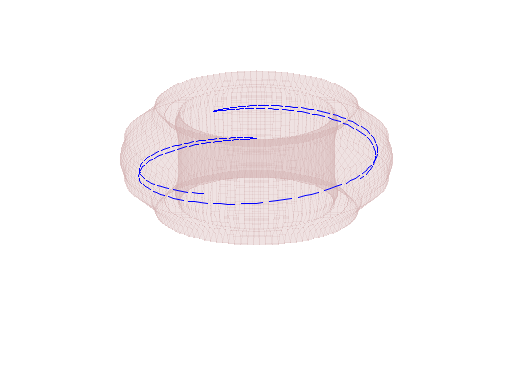
\includegraphics[width=0.8\textwidth,natwidth=610,natheight=642]{/home/yj/project_new/guiding_center_motion/fig14c/3d_orbit.png}
%  \includegraphics[scale=0.75]
  \caption{Three-dimensional illustration of the guidieng-center orbit of a
  trapped particle in a tokamak.}
\end{figure}

\subsection{Trapped particle fraction}

The trapped particle fraction $f_t$ is defined as the ratio of the number of
trapped particles to the total number of particles. Using spherical
coordinates in velocity space, the particle distribution function can be
written as $f = f (\mathbf{r}, v, \theta, \phi)$, where $\mathbf{r}$ is the
location vector in configuration space, $(v, \theta, \phi)$ is the spherical
coordinates in velocity space with $\theta$ being the pitch angle. Then the
trapped particle fraction $f_t$ is written as
\begin{equation}
  \label{16-6-29-1} f_t (\mathbf{r}) = 1 - \frac{2 \int_0^{\infty}
  \int_0^{\theta_{\tmop{tr}}} f (v, \theta, \varphi) v^2 \sin \theta d v d
  \theta d \phi}{\int_0^{\infty} \int_0^{\pi} f (v, \theta, \varphi) v^2 \sin
  \theta d v d \theta d \phi},
\end{equation}
where $\theta_{\tmop{tr}}$ is the critical pitch angle defined in Sec.
\ref{15-9-25-1}; the numerator of the fraction in Eq. (\ref{16-6-29-1}) is the
number of passing particles. Assuming $f$ is independent of $\phi$, then the
above equation is written as
\begin{equation}
  \label{15-9-24-p11} f_t (\mathbf{r}) = 1 - \frac{2 \int_0^{\infty}
  \int_0^{\theta_{\tmop{tr}}} f (v, \theta) 2 \pi v^2 \sin \theta d v d
  \theta}{\int_0^{\infty} \int_0^{\pi} f (v, \theta) 2 \pi v^2 \sin \theta d v
  d \theta} .
\end{equation}
If we further assume $f$ is independent of $\theta$, i.e., $f$ is isotropic in
velocity space, then Eq. (\ref{15-9-24-p11}) is written
\begin{eqnarray}
  f_t & = & 1 - \frac{4 \pi (1 - \cos \theta_{\tmop{tr}}) \int_0^{\infty} f
  v^2 d v}{4 \pi \int_0^{\infty} f v^2 d v} \nonumber\\
  & = & \cos \theta_{\tmop{tr}}  \label{15-9-24-p13}
\end{eqnarray}
The critical angle $\theta_{\tmop{tr}}$ in the zero-orbit-width approximation
is given by
\begin{equation}
  \sin^2 \theta_{\tmop{tr}} = \frac{B_I}{B_{\max}} .
\end{equation}
Using this in Eq. (\ref{15-9-24-p13}) yields
\begin{equation}
  \label{15-9-24-p10} f_t = \sqrt{1 - \frac{B_I}{B_{\max}}}
\end{equation}
In the large aspect ratio approximation and for particles that are initially
at the low-field-side of the midplane, Eq. (\ref{15-9-24-p10}) is written
\begin{equation}
  f_t = \sqrt{1 - \frac{R_0 - r}{R_0 + r}} = \sqrt{\frac{2 r}{R_0 + r}} .
\end{equation}
This is the result given in Wessson's book{\cite{wesson2004}}. Note that this
result is valid only for particles that are initially at the low-field-side of
the midplane. For particles that are initially located at the poloidal
location $\theta_p$, the trapped particles fraction is written
\begin{equation}
  \label{15-9-25-4} f_t = \sqrt{1 - \frac{R_0 - r}{R_0 + r \cos \theta_p}} =
  \sqrt{\frac{r (1 + \cos \theta_p) }{R_0 + r \cos \theta_p}},
\end{equation}
For $\theta_p = \pi$, i.e., at the high-field-side of the midplane, $f_t = 0$,
i.e., there is no trapped particles there.

Using Eq. (\ref{15-9-25-4}), the flux surface averaging of $f_t$, $\langle
f_t \rangle$, is written as
\begin{eqnarray*}
  \langle f_t \rangle & = & \frac{\oint f_t  \frac{1}{B_p} d l_p}{\oint
  \frac{1}{B_p} d l_p}\\
  & = & \frac{\oint \sqrt{\frac{r (1 + \cos \theta_p) }{R_0 + r \cos
  \theta_p}}  \frac{1}{B_p} d l_p}{\oint \frac{1}{B_p} d l_p}\\
  & = & \frac{\oint \sqrt{\frac{r (1 + \cos \theta_p) }{R_0 + r \cos
  \theta_p}}  \frac{1}{B_p} r d \theta}{\oint \frac{1}{B_p} r d \theta}
\end{eqnarray*}

\section{Numerical results of prompt loss of fast ions}

The initial distribtuion function of fast ions are assumed to take the
following form:
\begin{equation}
  \label{16-5-25-1} f (\psi, v, \lambda) = C \exp \left( -
  \frac{\psi}{\psi_{\tmop{scale}}} \right) \frac{1}{v^3 + v_{\tmop{crit}}^3} 
  \frac{1}{2} \tmop{erfc} \left( \frac{v - v_{\tmop{birth}}}{\Delta_v} \right)
  \exp \left( - \frac{(\lambda - \lambda_0)^2}{\Delta_{\lambda}^2} \right),
\end{equation}
where the constant $C$ is set to achieve desired stored energy of energetic
particles. Figure \ref{16-5-25-2} plots the time evolution of the loss
fraction due to the prompt loss (also called first orbit loss) in EAST\#48916
at 4.6s.

\

\

\

\begin{figure}[h]
  \includegraphics{/home/yj/project_new/guiding_center_motion/fig23b/p.eps}
  \caption{\label{16-5-25-2}Time evolution of fast ions loss fraction in EAST
  discharge \#48916 at 4.6s. Fast ions distribution function is given by Eq.
  (\ref{16-5-25-1}).}
\end{figure}


\[ d \Gamma = d V_s d V_v = R d R d Z d \phi 2 \pi \frac{B}{m} d
   v_{\parallel}' d \mu \]
\begin{equation}
  \frac{d \Gamma}{L_n^3 v_n^3} = \overline{R} d \overline{R} d \overline{Z} d
  \phi 2 \pi \frac{B}{m v_n^2} d \overline{v}_{\parallel}' d \mu =
  \overline{R} d \overline{R} d \overline{Z} d \phi 2 \pi \frac{
  \overline{B}}{m v_n^2 / B_n} d \overline{v}_{\parallel}' d \mu =
  \overline{R} d \overline{R} d \overline{Z} d \phi 2 \pi \overline{B} d
  \overline{v}_{\parallel}' d \overline{\mu}
\end{equation}
Marker's phase-space volume $V_j$

\section{Use constants of motion to determine orbit loss}

This section discusses determining the prompt loss of ions by using the
constants of motion. This work was motivated by Dr. Chengkang Pan, who shares
an office with me and recently (2014) published a NF paper discussing this
topic.

\subsection{Critical velocity for ions loss}

There are three constants of motion for the guiding center orbit, namely, the
canonical toroidal angular momentum $P_{\phi}$, the magnetic moment $\mu$, and
the total kinetic energey $\varepsilon$, which are given, respectively, by
\begin{equation}
  P_{\phi} = m \frac{g (\Psi) }{B} v \xi + Z e \Psi,
\end{equation}
\begin{equation}
  \mu = \frac{m}{B} v^2 (1 - \xi^2),
\end{equation}
\begin{equation}
  \varepsilon = \frac{1}{2} m v^2,
\end{equation}
where $g (\Psi) = R B_{\phi}$, $\xi$ is the cosine of the pitch angle of
guiding center velocity (with respect to the local magnetic field), $\Psi = R
A_{\phi}$ with $A_{\phi}$ being the toroidal component of the magnetic vector
potential, $Z e$ $(e > 0)$ and $m$ are the charge and mass of the ion,
respectively.

Next, we use the constraint of the three constants of motion to determine
whether an ion with a given initial condition can reach a boundary magnetic
surface labeled by $\Psi_a$. The initial conditions of an ion is denoted with
$(\Psi_0, B_0, v_0, \xi_0)$, where $\Psi_0$ lables the flux surface where the
particle is initially located, $B_0$ is the magnetic field strength at the
initial location of the guiding-center, $v_0$ and $\xi_0$ are the initial
velocity and pitch angle. The conditions of the particle when it reach the
boundary flux surface are denoted with $(\Psi_a, B_a, v_a, \xi_a)$. Then the
conservation of $P_{\phi}$ requires
\begin{equation}
  m \frac{g (\Psi_0)}{B_0} v_0 \xi_0 + e \Psi_0 = m \frac{g (\Psi_a)}{B_a} v_a
  \xi_a + e \Psi_a .
\end{equation}
Using the conservation of the kinetic energy, the above equation is written
\begin{equation}
  \label{11-20-p2} m v_0 \left( \frac{g (\Psi_0)}{B_0} \xi_0 - \frac{g
  (\Psi_a)}{B_a} \xi_a \right) = e (\Psi_a - \Psi_0) .
\end{equation}
Using the conservation of $\mu$, we obtain
\begin{equation}
  \frac{1 - \xi_a^2}{B_a} = \frac{1 - \xi_0^2}{B_0},
\end{equation}
which can be written
\begin{equation}
  \label{11-20-p1} \xi_a = \pm \sqrt{1 - \frac{B_a}{B_0} (1 - \xi_0^2)},
\end{equation}
Using Eq. (\ref{11-20-p1}), equation (\ref{11-20-p2}) is written
\begin{equation}
  \label{11-20-1} m v_0 \left[ \frac{g (\Psi_0)}{B_0} \xi_0 \mp \frac{g
  (\Psi_a)}{B_a} \sqrt{1 - \frac{B_a}{B_0} (1 - \xi_0^2)} \right] = e (\Psi_a
  - \Psi_0),
\end{equation}
which can be arranged in the form
\begin{equation}
  \label{11-20-p5} v_0 = \frac{e (\Psi_a - \Psi_0)}{m}  \left( \frac{g
  (\Psi_0)}{B_0} \xi_0 \mp \frac{g (\Psi_a)}{B_a} \sqrt{1 - \frac{B_a}{B_0} (1
  - \xi_0^2)} \right)^{- 1},
\end{equation}
Equation (\ref{11-20-p5}) gives the velocity $v_0$ needed for the particle to
reach the flux surface $\Psi_a$. The value of $v_0$ given by Eq.
(\ref{11-20-p5}) varies, depending on the value of $B_a$, i.e., depending on
the poloidal location on the boundary magnetic flux surface. By varying the
poloidal location on the boundary flux surface, we can obtain the minimum
value of $v_0$, $v_{0 \min}$, which is the minumu velocity for a particle with
the initial condition $(\Psi_0, B_0, \xi_0)$ to reach flux surface $\Psi_a$.

The above derivation does not distinguish between circulating particles and
trapped particles. Next, we distinguish between these two kinds of particles.
If the ion is a circulating one, then $v_{\parallel}$ does not change sign and
thus $\xi$ does not change sign either. In this case, equation
(\ref{11-20-p1}) is written
\begin{equation}
  \label{11-20-e10} \xi_a = \tmop{sign} (\xi_0) \sqrt{1 - \frac{B_a}{B_0} (1 -
  \xi_0^2)} .
\end{equation}
If the ion is a trapped one, then both signs $\pm$ in Eq. (\ref{11-20-p1}) are
possible.

To evaluate the minimum energy for the ions to be lost, we need choose a
equilibrium. Next, we give a simple large aspect ratio equilibrium.

\subsection{Large aspect ratio equilibrium}

Define $(r, \theta)$ coordinates by
\begin{equation}
  R (r, \theta) = \overline{R} + r \cos \theta,
\end{equation}
\begin{equation}
  Z (r, \theta) = r \sin \theta,
\end{equation}
The leading order equation of the Grad-Shafranov equation in $(r, \theta)$
coordinates is written (refer to my notes on tokamak equilibrium)


\begin{equation}
  \label{11-20-e3} \frac{1}{r}  \frac{d}{d r} r \frac{d \Psi}{d r} = - \mu_0
  \overline{R} J_{\phi} (r),
\end{equation}
which gives concentric circular flux surfaces centered at $(R = \overline{R},
Z = 0)$. Assume that $J_{\phi}$ is uniform distributed, i.e., $|J_{\phi} | = I
/ (\pi a^2)$, where $I$ is the total current within the flux surface $r = a$.
Further assume the current is in the opposite direction of $\nabla \phi$, then
$J_{\phi} = - I / (\pi a^2)$. Using this, Eq. (\ref{11-20-e3}) can be solved
to give
\begin{equation}
  \label{11-21-4} \Psi = \frac{\mu_0 I}{4 \pi a^2} \overline{R} r^2 .
\end{equation}
In $(r, \theta)$ corrdintates, the gradient of $\Psi$ is written
\begin{equation}
  \nabla \Psi = \frac{\mu_0 I}{2 \pi a^2} \overline{R} r \hat{\mathbf{e}}_r
\end{equation}
\begin{eqnarray}
  \mathbf{B}_p & = & \nabla \Psi \times \nabla \phi \nonumber\\
  & = &  \frac{\mu_0 I}{2 \pi a^2} \overline{R} r \hat{\mathbf{e}}_r \times
  \hat{\mathbf{e}}_{\phi} \frac{1}{R} \nonumber\\
  & = & \frac{\mu_0 I}{2 \pi a^2} \overline{R} \frac{r}{R}
  \hat{\mathbf{e}}_{\theta} \nonumber\\
  & = & \frac{\mu_0 I}{2 \pi a^2} \frac{r}{1 + \frac{r}{\overline{R}} \cos
  \theta} \hat{\mathbf{e}}_{\theta}  \label{11-19-e111}
\end{eqnarray}
where $\hat{\mathbf{e}}_{\theta}$ is the unit vector along the direction of
increassing $\theta$ (count-clockwise when looking along $\nabla \phi$).
Define $\rho = r / a$ and $\varepsilon = a / \overline{R}$, then Eq.
(\ref{11-19-e111}) is written
\[ \mathbf{B}_p = \frac{\mu_0 I}{2 \pi a} \frac{\rho}{1 + \rho \varepsilon
   \cos \theta} \hat{\mathbf{e}}_{\theta} . \]
The toroidal component of the magnetic field is written
\begin{equation}
  \label{11-19-p1} B_{\phi} = \frac{g (\Psi)}{R} = \frac{g
  (\Psi)}{\overline{R} + r \cos \theta} .
\end{equation}
Consider the case that $g (\Psi)$ is a contant function, $g (\Psi) = B_{\phi
0} \overline{R}$, then Eq. (\ref{11-19-p1}) is written
\begin{equation}
  B_{\phi} = \frac{B_{\phi 0}}{1 + \frac{r}{\overline{R}} \cos \theta} =
  \frac{B_{\phi 0}}{1 + \rho \varepsilon \cos \theta} .
\end{equation}

\begin{equation}
  B = \sqrt{B_{\phi}^2 + B_{\theta}^2} = \sqrt{\left( \frac{\mu_0 I}{2 \pi a}
  \rho \right)^2 + B_{\phi 0}^2} \frac{1}{1 + \rho \varepsilon \cos \theta} .
\end{equation}


\begin{figure}[h]
  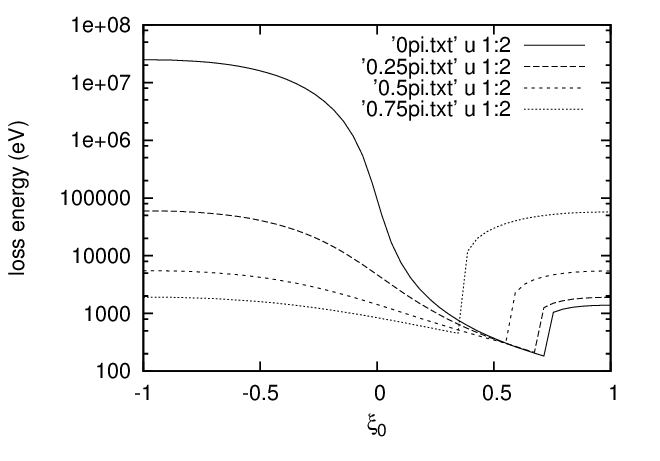
\includegraphics{/home/yj/project_new/orbit_loss_model/fig1/a.eps}
  \caption{Minimus loss energy as a function of the cosine of the launching
  pitch angle. $\rho = 0.98$}
\end{figure}

\

\

\

\

---------------------------------

The minimum value of $v_0$, denoted with $v_{0 \min}$, is reached when $\theta
= \pi$ or $\theta = 0$ depends on the $\pm$ in Eq. (\ref{11-19-1}).

\

\


\begin{equation}
  v_0 = \frac{e}{m R_0}  \frac{\mu_0 I}{4 \pi a^2} \overline{R} (a^2 - r^2)
  \left( \xi_0 \mp \tmop{sign} (\xi_0) \frac{\overline{R} + a}{\overline{R} +
  r} \sqrt{1 - \frac{\overline{R} + r}{\overline{R} + a} (1 - \xi_0^2)}
  \right)^{- 1} .
\end{equation}


\


\begin{equation}
  v_{0 \min} (\xi_0) = \max (\min (v_0 (\xi_0, \theta)), 0)
\end{equation}


\

\

\

\

(in practice $\psi_a$ is usually different from the actual poloidal flux
$\Psi_p$ and is related to $\Psi_p$ by $\psi_a = \pm | \Psi_p | / 2 \pi + C$,
where $C$ is a constant)

\

\

\

\

Circulating region
\begin{equation}
  1 - \xi^2 < \frac{B_{\min}}{B_{\max}}
\end{equation}
we consider the confinement of the particles. The method is to determine
whether the particles can reach a boundary flux surface by making use of the
three constants of the motion. The boundary flux surface is labled by
$\psi_a$, where $\psi_a$ is the poloidal flux within that flux surface.

\

Next examine what the conservation of $P_{\phi}$, $\mu$, and $\varepsilon$
requires if the particle can reach the boundary surface.

\

Consider the case $\nabla \Psi$ is pointing from the magnetic axis to the
boundary flux surface, i.e., $\Psi$ is increasing from the magnetic axis to
the boundary magnetic surface. Since $\mathbf{B}_p = \nabla \Psi \times \nabla
\phi$, the case corresponds to that $B_p$ is count clockwise when the observer
looks along the direction of $\nabla \phi$.

\

Using the coordinates transformation, equation (\ref{11-21-4}) can be further
written
\begin{equation}
  \Psi = \frac{\mu_0 I}{4 \pi a^2} \overline{R} [(R - \overline{R})^2 + Z^2] .
\end{equation}
Then the gradiant of $\Psi$ is written
\begin{equation}
  \nabla \Psi = \frac{\mu_0 I}{4 \pi a^2} \overline{R} [2 (R - \overline{R})
  \hat{\mathbf{R}} + 2 Z \hat{\mathbf{Z}}]
\end{equation}
and the poloidal magnetic field is written
\begin{eqnarray}
  \mathbf{B}_p & = & \nabla \Psi \times \nabla \phi \nonumber\\
  & = & \frac{\mu_0 I}{4 \pi a^2} \overline{R} [2 (R - \overline{R})
  \hat{\mathbf{R}} + 2 Z \hat{\mathbf{Z}}] \times \frac{1}{R}
  \hat{\mathbf{\phi}} \nonumber\\
  & = & \frac{\mu_0 I}{4 \pi a^2} \overline{R} \frac{1}{R} [2 (R -
  \overline{R}) \hat{\mathbf{Z}} - 2 Z \hat{\mathbf{R}}] \nonumber\\
  & = & \frac{\mu_0 I}{4 \pi a^2} \overline{R} \frac{2 r}{R} [\cos \theta
  \hat{\mathbf{Z}} - \sin \theta \hat{\mathbf{R}}] \nonumber\\
  & = & \frac{\mu_0 I}{4 \pi a^2} \overline{R} \frac{2 r}{R}
  \hat{\mathbf{\theta}}, \nonumber\\
  & = & \frac{\mu_0 I}{4 \pi a^2} \frac{2 r}{1 + \frac{r}{\overline{R}} \cos
  \theta} \hat{\mathbf{\theta}} . 
\end{eqnarray}
where $\hat{\mathbf{\theta}}$ is the unit vector along the direction of
increassing $\theta$ (count-clockwise when looking along $\nabla \phi$).

\

\

\

\section{Equations of guiding-center motion---outdated, will be deleted}

YJ's remark: This section is outdated because I have found a more accurate
form of the equations of the guiding center motion, as given in Sec.
\ref{5-15-e1}. Besides to be more accurate, the new form is compact and
suitable for numerical implemention

The equations for the guiding center motion are given by (refer to my note
``collisionless\_drift\_kinetic\_equation.tm'')
\begin{equation}
  \label{11-17-7} \dot{\mathbf{X}} = v_{\parallel} \mathbf{b}+
  \frac{1}{\Omega} \mathbf{b} \times \left( \frac{\mu}{m} \nabla B +
  v_{\parallel}^2 \mathbf{\kappa} \right),
\end{equation}
and
\begin{equation}
  \label{1-28-p1} \dot{v_{\parallel}} = - \frac{\mu}{m} \mathbf{b} \cdot
  \nabla B + v_{\parallel} \mathbf{\kappa} \cdot \dot{\mathbf{X}},
\end{equation}
where $\mu \equiv m v_{\perp}^2 / (2 B)$, $\mathbf{b}=\mathbf{B}/ B$. The term
$v_{\parallel} \mathbf{\kappa} \cdot \dot{\mathbf{X}}$ in Eq. (\ref{1-28-p1})
can be further simplified by using Eq. (\ref{11-17-7}), which gives
\begin{equation}
  \label{11-17-8} \dot{v_{\parallel}} = - \frac{\mu}{m} \mathbf{b} \cdot
  \nabla B + \frac{v_{\parallel} \mu}{m \Omega} \mathbf{\kappa} \cdot
  \mathbf{b} \times \nabla B
\end{equation}
where use has been made of that the curvature $\mathbf{\kappa}$ is
perpendicular to $\mathbf{b}$.

[Benchmark: In GTC simulation (refer to H. Zhang's paper{\cite{zhang2010}}),
the time derivative of $v_{\parallel}$ is given by
\begin{equation}
  \dot{v}_{\parallel} = - \frac{\mathbf{B}+ B v_{\parallel} / \Omega_{\alpha}
  \nabla \times \mathbf{b}}{m B} \cdot \mu \nabla B
\end{equation}
\begin{equation}
  \label{1-31-1} \Longrightarrow \dot{v}_{\parallel} = - \frac{\mu}{m}
  \mathbf{b} \cdot \nabla B - \frac{v_{\parallel} \mu}{m \Omega} \nabla \times
  \mathbf{b} \cdot \nabla B,
\end{equation}
Next, I prove Eq. (\ref{11-17-8}) is equivalent to Eq. (\ref{1-31-1}). Using
$\mathbf{\kappa} \equiv \mathbf{b} \cdot \nabla \mathbf{b}= -\mathbf{b} \times
\nabla \times \mathbf{b}$, the second term on the right-hand side of Eq.
(\ref{11-17-8}) is written as
\begin{eqnarray}
  \frac{v_{\parallel} \mu}{m \Omega} \mathbf{\kappa} \cdot \mathbf{b} \times
  \nabla B & = & - \frac{v_{\parallel} \mu}{m \Omega} (\mathbf{b} \times
  \nabla \times \mathbf{b}) \cdot (\mathbf{b} \times \nabla B) \nonumber\\
  & = & - \frac{v_{\parallel} \mu}{m \Omega} \nabla \times \mathbf{b} \cdot
  \nabla B + \frac{v_{\parallel} \mu}{m \Omega} (\mathbf{b} \cdot \nabla B)
  (\nabla \times \mathbf{b} \cdot \mathbf{b}) \nonumber\\
  & \approx & - \frac{v_{\parallel} \mu}{m \Omega} \nabla \times \mathbf{b}
  \cdot \nabla B + 0,  \label{1-29-1}
\end{eqnarray}
where in obtaining the last equality, use has been made of that $\nabla \times
\mathbf{b} \cdot \mathbf{b} \approx 0$ (note that this is correct to the order
considered here, I will discuss this later). Using \ Eq. (\ref{1-29-1}) in Eq.
(\ref{11-17-8}) yields
\begin{equation}
  \label{1-28-1} \dot{v_{\parallel}} = - \frac{\mu}{m} \mathbf{b} \cdot \nabla
  B - \frac{v_{\parallel} \mu}{m \Omega} \nabla \times \mathbf{b} \cdot \nabla
  B,
\end{equation}
which is identical with Eq. (\ref{1-31-1}).]

\subsection{Equations of guiding center motion in cylindrical coordinates-old,
will be deleted}

In the cylindrical coordinates $(R, \phi, Z)$, the location vector is written
as
\begin{equation}
  \mathbf{X}= R \hat{\mathbf{e}}_R + Z \hat{\mathbf{e}}_Z .
\end{equation}
Using this, we obtain
\begin{equation}
  \Rightarrow \dot{\mathbf{X}} = \dot{R} \hat{\mathbf{e}}_R + R \dot{\phi}
  \hat{\mathbf{e}}_{\phi} + \dot{Z} \hat{\mathbf{e}}_Z
\end{equation}
Substituting this into the equation of motion gives
\begin{equation}
  \label{11-17-2} \dot{R} \hat{\mathbf{e}}_R + R \dot{\phi}
  \hat{\mathbf{e}}_{\phi} + \dot{Z} \hat{\mathbf{e}}_Z = v_{\parallel}
  \mathbf{b}+ \frac{1}{\Omega} \mathbf{b} \times \left( \frac{\mu}{m} \nabla B
  + v_{\parallel}^2 \mathbf{\kappa} \right) .
\end{equation}
The $\hat{\mathbf{e}}_R$ component of the above equation is written as
\begin{equation}
  \label{11-17-1} \dot{R} = v_{\parallel} b_R + \hat{\mathbf{e}}_R \cdot
  \frac{1}{\Omega} \mathbf{b} \times \left( \frac{\mu}{m} \nabla B +
  v_{\parallel}^2 \mathbf{\kappa} \right) .
\end{equation}
Using
\begin{eqnarray}
  \hat{\mathbf{e}}_R \cdot \frac{1}{\Omega} \mathbf{b} \times \frac{\mu}{m}
  \nabla B & = & \frac{\mu}{m \Omega} \hat{\mathbf{e}}_R \cdot \mathbf{b}
  \times \nabla B \nonumber\\
  & = & \frac{\mu}{m \Omega} \hat{\mathbf{e}}_R \cdot (b_R \hat{\mathbf{e}}_R
  + b_Z \hat{\mathbf{e}}_Z + b_{\phi} \hat{\mathbf{e}}_{\phi}) \times \left(
  \frac{\partial B}{\partial R} \hat{e}_R + \frac{\partial B}{\partial Z}
  \hat{e}_Z \right) \nonumber\\
  & = & \frac{\mu}{m \Omega} b_{\phi}  \frac{\partial B}{\partial Z} 
\end{eqnarray}
and
\begin{eqnarray}
  \hat{\mathbf{e}}_R \cdot \frac{1}{\Omega} \mathbf{b} \times v_{\parallel}^2
  \mathbf{\kappa} & = & \frac{v_{\parallel}^2}{\Omega} \hat{\mathbf{e}}_R
  \cdot (\mathbf{b} \times \mathbf{\kappa}) \nonumber\\
  & = & \frac{v_{\parallel}^2}{\Omega} \hat{\mathbf{e}}_R \cdot (b_R
  \hat{\mathbf{e}}_R + b_Z \hat{\mathbf{e}}_Z + b_{\phi}
  \hat{\mathbf{e}}_{\phi}) \times (\kappa_R \hat{e}_R + \kappa_Z \hat{e}_Z +
  \kappa_{\phi} \hat{e}_{\phi}) \nonumber\\
  & = & \frac{v_{\parallel}^2}{\Omega} (- b_Z \kappa_{\phi} + b_{\phi}
  \kappa_Z), 
\end{eqnarray}
Eq. (\ref{11-17-1}) is written as
\begin{equation}
  \label{11-17-6} \dot{R} = v_{\parallel} b_R + \frac{\mu}{m \Omega} b_{\phi} 
  \frac{\partial B}{\partial Z} + \frac{v_{\parallel}^2}{\Omega} (- b_Z
  \kappa_{\phi} + b_{\phi} \kappa_Z) .
\end{equation}
Equation (\ref{11-17-6}) is used in my numerical code. The
$\hat{\mathbf{e}}_Z$ component of Eq. (\ref{11-17-2}) is written as
\begin{equation}
  \label{11-17-4} \dot{Z} = v_{\parallel} b_Z + \hat{\mathbf{e}}_Z \cdot
  \frac{1}{\Omega} \mathbf{b} \times \left( \frac{\mu}{m} \nabla B +
  v_{\parallel}^2 \mathbf{\kappa} \right) .
\end{equation}
Using
\begin{eqnarray}
  \hat{\mathbf{e}}_Z \cdot \frac{1}{\Omega} \mathbf{b} \times \frac{\mu}{m}
  \nabla B & = & \frac{\mu}{m \Omega} \hat{\mathbf{e}}_Z \cdot \mathbf{b}
  \times \nabla B \nonumber\\
  & = & \frac{\mu}{m \Omega} \hat{\mathbf{e}}_Z \cdot (b_R \hat{\mathbf{e}}_R
  + b_Z \hat{\mathbf{e}}_Z + b_{\phi} \hat{\mathbf{e}}_{\phi}) \times \left(
  \frac{\partial B}{\partial R} \hat{e}_R + \frac{\partial B}{\partial Z}
  \hat{e}_Z \right) \nonumber\\
  & = & - \frac{\mu}{m \Omega} b_{\phi}  \frac{\partial B}{\partial R} 
\end{eqnarray}
and
\begin{eqnarray}
  \hat{\mathbf{e}}_Z \cdot \frac{1}{\Omega} \mathbf{b} \times v_{\parallel}^2
  \mathbf{\kappa} & = & \frac{v_{\parallel}^2}{\Omega} \hat{\mathbf{e}}_Z
  \cdot \mathbf{b} \times \mathbf{\kappa} \nonumber\\
  & = & \frac{v_{\parallel}^2}{\Omega} \hat{\mathbf{e}}_Z \cdot (b_R
  \hat{\mathbf{e}}_R + b_Z \hat{\mathbf{e}}_Z + b_{\phi}
  \hat{\mathbf{e}}_{\phi}) \times (\kappa_R \hat{e}_R + \kappa_Z \hat{e}_Z +
  \kappa_{\phi} \hat{e}_{\phi}) \nonumber\\
  & = & \frac{v_{\parallel}^2}{\Omega} (b_R \kappa_{\phi} - b_{\phi}
  \kappa_R), 
\end{eqnarray}
Eq. (\ref{11-17-4}) is written as
\begin{equation}
  \label{11-17-5} \dot{Z} = v_{\parallel} b_Z - \frac{\mu}{m \Omega} b_{\phi} 
  \frac{\partial B}{\partial R} + \frac{v_{\parallel}^2}{\Omega} (b_R
  \kappa_{\phi} - b_{\phi} \kappa_R) .
\end{equation}
Equation (\ref{11-17-5}) is used in my numerical code.

Next we consider the equation for the time evolution of $v_{\parallel}$, Eq.
(\ref{11-17-8}), i.e.,
\begin{equation}
  \label{5-9-a1} \dot{v_{\parallel}} = - \frac{\mu}{m} \mathbf{b} \cdot \nabla
  B + \frac{v_{\parallel} \mu}{m \Omega} \mathbf{\kappa} \cdot \mathbf{b}
  \times \nabla B.
\end{equation}
The first term of on the right-hand side of Eq. (\ref{5-9-a1}) can be written
as
\begin{eqnarray}
  - \frac{\mu}{m} \mathbf{b} \cdot \nabla B & = & - \frac{\mu}{m}  (b_R
  \hat{e}_R + b_Z \hat{e}_Z + b_{\phi} \hat{e}_{\phi}) \cdot \left(
  \frac{\partial B}{\partial R} \hat{e}_R + \frac{\partial B}{\partial Z}
  \hat{e}_Z \right) \nonumber\\
  & = & - \frac{\mu}{m}  \left( b_R  \frac{\partial B}{\partial R} + b_Z 
  \frac{\partial B}{\partial Z} \right) . 
\end{eqnarray}
The second term on the right-hand side of Eq. (\ref{5-9-a1}) can be written as
\begin{eqnarray}
  \mathbf{\kappa} \cdot [\mathbf{b} \times \nabla B] & = & (\kappa_R \hat{e}_R
  + \kappa_Z \hat{e}_Z + \kappa_{\phi} \hat{e}_{\phi}) \cdot \left[ (b_R
  \hat{e}_R + b_Z \hat{e}_Z + b_{\phi} \hat{e}_{\phi}) \times \left(
  \frac{\partial B}{\partial R} \hat{e}_R + \frac{\partial B}{\partial Z}
  \hat{e}_Z \right) \right] \nonumber\\
  & = & (\kappa_R \hat{e}_R + \kappa_Z \hat{e}_Z + \kappa_{\phi}
  \hat{e}_{\phi}) \cdot \left[ - b_R \frac{\partial B}{\partial Z}
  \hat{e}_{\phi} + b_Z \frac{\partial B}{\partial R} \hat{e}_{\phi} - b_{\phi}
  \frac{\partial B}{\partial R} \hat{e}_Z + b_{\phi} \frac{\partial
  B}{\partial Z} \hat{e}_R \right] \nonumber\\
  & = & \kappa_R b_{\phi}  \frac{\partial B}{\partial Z} - \kappa_Z b_{\phi} 
  \frac{\partial B}{\partial R} + \kappa_{\phi} \left( b_Z \frac{\partial
  B}{\partial R} - b_R \frac{\partial B}{\partial Z} \right) . 
\end{eqnarray}
Using these results, Eq. (\ref{5-9-a1}) is written as
\begin{equation}
  \label{11-19-1} \dot{v_{\parallel}} = - \frac{\mu}{m}  \left( b_R 
  \frac{\partial B}{\partial R} + b_Z  \frac{\partial B}{\partial Z} \right) +
  \frac{\mu v_{\parallel}}{m \Omega} \left[ \kappa_R b_{\phi}  \frac{\partial
  B}{\partial Z} - \kappa_Z b_{\phi}  \frac{\partial B}{\partial R} +
  \kappa_{\phi} \left( b_Z \frac{\partial B}{\partial R} - b_R \frac{\partial
  B}{\partial Z} \right) \right] .
\end{equation}
Equation (\ref{11-19-1}) is used in my numerical code.

Next consider the $\hat{\mathbf{e}}_{\phi}$ component of Eq. (\ref{11-17-2}),
which is written as
\begin{equation}
  \label{1-31-p1} R \dot{\phi} = v_{\parallel} b_{\phi} + \frac{1}{\Omega}
  \hat{\mathbf{e}}_{\phi} \cdot \left[ \mathbf{b} \times \left( \frac{\mu}{m}
  \nabla B + v_{\parallel}^2 \mathbf{\kappa} \right) \right] .
\end{equation}
Using
\begin{eqnarray}
  \frac{1}{\Omega} \hat{\mathbf{e}}_{\phi} \cdot \left( \mathbf{b} \times
  \frac{\mu}{m} \nabla B \right) & = & \frac{\mu}{\Omega m}
  \hat{\mathbf{e}}_{\phi} \cdot (\mathbf{b} \times \nabla B) \nonumber\\
  & = & \frac{\mu}{\Omega m} \hat{\mathbf{e}}_{\phi} \cdot \left[ (b_R
  \hat{\mathbf{e}}_R + b_Z \hat{\mathbf{e}}_Z) \times \left( \frac{\partial
  B}{\partial R} \hat{e}_R + \frac{\partial B}{\partial Z} \hat{e}_Z \right)
  \right] \nonumber\\
  & = & \frac{\mu}{\Omega m} \left( - b_R  \frac{\partial B}{\partial Z} +
  b_Z  \frac{\partial B}{\partial R} \right), 
\end{eqnarray}
and
\begin{eqnarray}
  \frac{v_{\parallel}^2}{\Omega} \hat{\mathbf{e}}_{\phi} \cdot \mathbf{b}
  \times \mathbf{\kappa} & = & \frac{v_{\parallel}^2}{\Omega}
  \hat{\mathbf{e}}_{\phi} \cdot (b_R \hat{\mathbf{e}}_R + b_Z
  \hat{\mathbf{b}}_Z) \times (\kappa_R \hat{\mathbf{e}}_R + \kappa_Z
  \hat{\mathbf{b}}_Z) \nonumber\\
  & = & \frac{v_{\parallel}^2}{\Omega} (- b_R \kappa_Z + b_Z \kappa_R), 
\end{eqnarray}
Eq. (\ref{1-31-p1}) is written as
\begin{equation}
  \label{1-31-p2} R \dot{\phi} = v_{\parallel} b_{\phi} + \frac{\mu}{\Omega m}
  \left( - b_R  \frac{\partial B}{\partial Z} + b_Z  \frac{\partial
  B}{\partial R} \right) + \frac{v_{\parallel}^2}{\Omega} (- b_R \kappa_Z +
  b_Z \kappa_R) .
\end{equation}
Equation (\ref{1-31-p2}) (in normalized form) is used in my numerical code.

\

\

\begin{thebibliography}{1}
  \bibitem[1]{todo2006}Y.~Todo. {\newblock}Properties of energetic-particle
  continuum modes destabilized by energetic ions with beam-like velocity
  distributions. {\newblock}\tmtextit{Phys. Plasmas (1994-present)}, 13(8):--,
  2006.
  
  \bibitem[2]{wesson2004}John Wesson. {\newblock}\tmtextit{Tokamaks}.
  {\newblock}Oxford University Press, 2004.
  
  \bibitem[3]{lin1995}Z.~Lin, W.~M. Tang, and W.~W. Lee.
  {\newblock}Gyrokinetic particle simulation of neoclassical transport.
  {\newblock}\tmtextit{Physics of Plasmas}, 2(8):2975, 1995.
  
  \bibitem[4]{boozer2005}Allen~H. Boozer. {\newblock}Physics of magnetically
  confined plasmas. {\newblock}\tmtextit{Rev. Mod. Phys.}, 76:1071--1141, Jan
  2005.
  
  \bibitem[5]{wang1998}Shaojie Wang. {\newblock}Finite bootstrap current
  density and finite neoclassical reduction of electrical conductivity at the
  magnetic axis of a tokamak. {\newblock}\tmtextit{Phys. Fluids},
  5(9):3319--3324, 1998.
  
  \bibitem[6]{zhang2010}H.~S. Zhang, Z.~Lin, I.~Holod, X.~Wang, Y.~Xiao, and
  W.~L. Zhang. {\newblock}Gyrokinetic particle simulation of beta-induced
  alfv{\'e}n eigenmode. {\newblock}\tmtextit{Phys. Plasmas}, 17(11):112505,
  2010.
\end{thebibliography}

\end{document}
